
\documentclass[12pt, oneside, a4paper]{enetcom-pfe-report}

\graphicspath{{images/}}

%%%%%%%%%%%%%%%%%%%%%%%%%%%%%%%%%%%%%%%%%%%%%%%%%%%%%%%%%%%
% Include useful commands
%%%%%%%%%%%%%%%%%%%%%%%%%%%%%%%%%%%%%%%%%%%%%%%%%%%%%%%%%%%
\newcommand{\reportAuthor} {%
  Prénom \textsc{NOM}%
}

\newcommand{\reportTitle} {%
   TITRE DU PROJET \\ Title%
}

\newcommand{\reportSubject} {%
   TITRE DU PROJET \\ Title%
}

\newcommand{\dateSoutenance} {%
  jj/mm/aaaa%
}

\newcommand{\studyDepartment} {%
  Génie Systèmes Électroniques 
et Communication%
}

\newcommand{\ENETCOM} {%
  École nationale d'électronique et des télécommunications de Sfax%
}

\newcommand{\codePFE} {% Reference %
}

\newcommand{\juryPresident} {%
  Mr Foulen \textsc{Fouleni}%
}
\newcommand{\juryPresidentDesc} {%
  President%
}

\newcommand{\juryMemberOne} {%
  Ms Foulena \textsc{Foulenia}%
}
\newcommand{\juryMemberOneDesc} {%
  Supervisor %Mentor
}

\newcommand{\juryMemberTwo} {%
  Mr Foulen \textsc{Fouleni}%
}
\newcommand{\juryMemberTwoDesc} {%
  Reviewer% Examiner, Reporter
}

\newcommand{\specialcell}[1]{%
  \begin{tabularx}{\textwidth}{@{}X@{}}#1\end{tabularx}%
}


%%%%%%%%%%%%%%%%%%%%%%%%%%%%%%%%%%%%%%%%%%%%%%%%%%%%%%%
% Add your own commands here
%%%%%%%%%%%%%%%%%%%%%%%%%%%%%%%%%%%%%%%%%%%%%%%%%%%%%%%
\newcommand{\MyCommand} {%
  Does nothing really%
}

\hypersetup{
  pdftitle={\reportTitle~-~\reportSubject},%
  pdfauthor={\reportAuthor},%
  pdfsubject={\reportSubject},%
  pdfkeywords={report} {internship} {pfe} {enentcom}
}
\dominitoc
\begin{document}
	\sloppy
    \thispagestyle{empty}
\begin{titlepage}
\begin{center}

%%%%%%%%%%%%%%%%%%%%%%%%%%%%%%%%%%%%%%%%%%%%%%%
% THE HEADER
%%%%%%%%%%%%%%%%%%%%%%%%%%%%%%%%%%%%%%%%%%%%%%%
{%
  \fontsize{9pt}{9pt}\selectfont%
  \begin{tabularx}{\textwidth}{ @{} p{0.35\textwidth} @{} p{0.02\textwidth} @{} p{0.3\textwidth} @{} p{0.02\textwidth} @{} p{0.35\textwidth} @{} }
    %
    %
    %
    % line 1
    \centering%
    {\fontsize{11}{1}\selectfont UNIVERSITÉ NORBERT ZONGO}
    \begin{spacing}{1}
    \end{spacing}
    \begin{spacing}{0.05}
    \noindent
    \rule{50pt}{0.75pt}\\
    \rule{50pt}{0.75pt}
    \end{spacing}
    \begin{spacing}{1.4}
    \end{spacing}
    {\fontsize{12}{1}\selectfont UFR-Sciences et Technologies}
    \begin{spacing}{1}
    \end{spacing}
    \begin{spacing}{0.05}
    \noindent
    \rule{50pt}{0.75pt}\\
    \rule{50pt}{0.75pt}
    \end{spacing}
  
    &%
    % Column 2 is empty 
    &%
    % Column 3
    \centering%
    \multirow{2}{\linewidth}{%
      \centering%
      
\includegraphics[width=5cm, height=4cm]{universite-norbert-zongo-removebg-preview.png}%
    }%
    &%
    % Column 4 is empty 
    &%
    % Column 5
    \centering%
    {\fontsize{12}{1}\selectfont Burkina Faso}\\%
    \begin{spacing}{1}
    \end{spacing}
    \begin{spacing}{0.05}
    \noindent
    \rule{50pt}{0.75pt}\\
    \rule{50pt}{0.75pt}
    \end{spacing}
    \begin{spacing}{1.4}
    \end{spacing}
    {\fontsize{12}{1}\selectfont \textit{Unité - Progrès - Justice}}%

    \tabularnewline%
    %
    %
    %
    % Line 2
    \centering%
    {\fontsize{12}{1}\selectfont Département d'Informatique}\\%
    &%
    % Column 2 is empty 
    &%
    % Column 3 is empty (contains the ENETCOM logo)
    &%
    % Column 4 is empty 
    &%
    {\fontsize{12}{1}\selectfont Année académique: 2022 - 2023}\\%
    \centering%
    \textbf{%
    }
     %
     \vspace{0.90cm}
    \tabularnewline%
    \arrayrulecolor{reportType}%
    \specialrule{0.75pt}{2pt}{0pt}%
    \specialrule{2.00pt}{1pt}{0pt}%
  \end{tabularx}
}


%%%%%%%%%%%%%%%%%%%%%%%%%%%%%%%%%%%%%%%%%%%%%%%
% THE PAGE CONTENT
%%%%%%%%%%%%%%%%%%%%%%%%%%%%%%%%%%%%%%%%%%%%%%%
\vspace{20pt}

{\fontsize{18}{1}\selectfont RAPPORT DE PROJET TUTORÉ}

\vspace{15pt}

\begin{tcolorbox}[
    enhanced,
    colback={rgb:red,10;green,132;blue,225}, % couleur de fond
    colframe={rgb:red,10;green,132;blue,225}, % couleur de la bordure rgba(10, 132, 255, 1)
    fontupper=\large\color{white}, % police large et couleur blanche
    arc=0pt, % pas de coins arrondis
    coltext=white, % couleur du texte blanc
    center, % centrage du texte
]
\begin{center}
Pour l’obtention du diplôme de Licence
\end{center}
\end{tcolorbox}

\vspace{20pt}

{\fontsize{14}{1}\selectfont Filière: Mathématique-Physique-Chimie-Informatique}

\vspace{15pt}

{\fontsize{14}{1}\selectfont Option: Informatique}

\vspace{20pt}

\begin{tcolorbox}[
    enhanced,
    colback=gray!20, % couleur de fond
    colframe=black, % couleur de la bordure
    rounded corners, % coins arrondis
    fontupper=\fontsize{20}{24}\selectfont\bfseries, % police et taille du texte
    drop shadow % effet d'ombre
]
\begin{center}
Prédiction de réussite de licence économie à l'UNZ par l'intelligence artificielle \\ 

\end{center}
\end{tcolorbox}

\vspace{30pt}

{\fontsize{16}{1}\selectfont Présenté par : \textbf{Paroguenssaongo Roméo SAWADOGO}}

\vspace{10pt}
{\fontsize{16}{1}\selectfont INE : \textbf{E01762820201}}

\end{center}

\vspace{30pt}
{\fontsize{16}{1}\selectfont Encadré par:}\\
\vspace{2pt}

{\fontsize{14}{1}\selectfont \textbf{Frédéric Tounwendyam OUEDRAOGO}}, Professeur titulaire en informatique à\\ \hspace*{260pt} l'Université Norbert Zongo\\
\vspace{2pt}

{\fontsize{14}{1}\selectfont \textbf{Paonouor SOMÉ}}, Directeur des Services Informatiques de l'Université Norbert Zongo\\ 

\vspace{25pt}

\begin{center}
Juin 2024
\end{center}
\end{titlepage}

    \doublespacing{}% Double spacing between lines
    \pagenumbering{roman}% i ii iii iv ...
    
    \addstarredchapter{DÉDICACE}
%\addcontentsline{toc}{chapter}{DEDICATION}
%\adjustmtc
%
%For all they have endured to satisfy all my needs and wishes\begin{center}
\nopagebreak{%
\vspace*{10cm}
  \raggedright\hspace{5,75cm} \huge {À mes très chers parents}\\
  \vspace{-2cm}
}

    \chapter*{REMERCIEMENTS}
\addstarredchapter{REMERCIEMENTS}
%\addcontentsline{toc}{chapter}{REMERCIEMENT}
%\adjustmtc
\thispagestyle{MyStyle}
%\sloppy

Je tiens tout d'abord à remercier très sincèrement mon encadreur, Pr Frédéric OUEDRAOGO, Professeur titulaire à l'UNZ, pour son accompagnement, sa disponibilité, ses précieux conseils et suggestions qui ont été d'un grand intérêt pour la réussite de ce travail.

Ensuite, je remercie mon co-encadreur M. Paonouor SOMÉ, Directeur des  Services Informatiques (DSI) de l'UNZ, qui m'a guidé durant mes travaux de recherche malgré ses multiples occupations.

Je tiens aussi à remercier le corps professoral de l’UNZ, en particulier celui de l’UFR-ST dont les enseignants m’ont permis d’acquérir les connaissances nécessaires à la réalisation de ce projet.

Je remercie de plus mes frères et sœurs, notamment Richard SAWADOGO, Marietta SAWADOGO, Odile TARBANGDO et mes camarades de l'UFR-ST, particulièrement ceux de la filière d'informatique, pour leur soutien moral et spirituel.

Enfin, je remercie tous les membres du personnel administratif de l'UFR-ST qui m'a soutenu à travers leur conseil dans mes études, en particulier mon très cher parrain M. Narcisse OUEDRAOGO, Dr Moustapha BIKIENGA, chef de département informatique, M. Maxime IDOGO, chef de service de la scolarité de l'UFR-ST et Mme Catherine TOÉ/KONATÉ, secrétaire principale de l'UFR-ST.
    
    \chapter*{PRÉAMBULE}
\addstarredchapter{PRÉAMBULE}
%\addcontentsline{toc}{chapter}{REMERCIEMENT}
%\adjustmtc
\thispagestyle{MyStyle}

L'Université Norbert Zongo (UNZ), anciennement l'Université de Koudougou, a été créée par décret N° 2005-460/PRES/PM/ MESSRS/MFB du 31 août 2005, résultant de la transformation de l'École Normale Supérieure de Koudougou (ENSK). Son appellation actuelle, décidée lors du Conseil des Ministres du 21 juillet 2017, rend hommage à Norbert Zongo, un journaliste émérite dont l'engagement pour la bonne gouvernance demeure exemplaire. L'UNZ est implantée au bord de l'Avenue Maurice Yaméogo (Route Nationale N°14) à Koudougou, chef-lieu de la province du Boulkiemdé et de la région du Centre-Ouest. Sa devise, "Scientia Excelle Ut Melius Servias", reflète son engagement pour l'excellence académique et le service à la communauté.

Conformément aux statuts approuvés par le décret N° 2017-0144 PRES/ PM/MESRSI/MINEFID du 22 mars 2017, l'UNZ est un Établissement Public de l'État à caractère Scientifique, Culturel et Technique, jouissant d'une personnalité morale et d'une autonomie scientifique, pédagogique, administrative et financière. Ses structures administratives, techniques et de gestion comprennent le Conseil d'Administration, le Conseil de la Formation et de la Vie Universitaire, le Conseil Scientifique, la Présidence, ainsi que les établissements d'enseignement, de formation et les centres de recherche.\\
Elle dispose en son sein de sept établissements, à savoir :
\begin{itemize}
	\item[\ding{118}] l'UFR-SEG;
	\item[\ding{118}] l'UFR-LSH;
	\item[\ding{118}] l'UFR-ST;
	\item[\ding{118}] l'IUT;
	\item[\ding{118}] l'ED-ST;
	\item[\ding{118}] l'ED-LACOSHS;
	\item[\ding{118}] le CPU
\end{itemize}
Parmi les sept établissements abrités par l'UNZ, nous avons eu le privilège de suivre notre formation à l'UFR-ST, créée en 2014. Cette unité s'inscrit dans le cadre du système LMD et offre une gamme variée de formations dans les domaines scientifiques et technologiques.\\
L’UFR-ST est un établissement supérieur d’enseignement général dont l’objectif est de former les étudiants dans les domaines scientifiques et technologiques. Dans le cadre du système LMD, elle prépare les étudiants à des Licences, des Masters et des Doctorats dans les filières suivantes :
\begin{itemize}
   \item[\ding{118}] MPCI : ce parcours aboutit aux licences en Mathématique, Physique, Chimie et Informatique, puis au Master et au Doctorat.
    
    \item[\ding{118}] SVT : ce parcours aboutit aux licences en Biologie Générale et Biochimie Fondamentale, puis au Master et au Doctorat.
\end{itemize}
L'accès à ces différentes filières se fait à travers des orientations effectuées via la plate-forme Campus Faso. Pour le cycle Master et le cycle Doctorat, la sélection se fait également via cette plateforme, sur la base d'un dossier de candidature.\\
Le cycle LMD favorise également la réalisation de projets tutorés dans la spécialité informatique, offrant aux étudiants en fin de cycle de licence une expérience pratique et leur permettant de développer leurs compétences.
Dans cette optique, nous avons suivi un stage de trois mois à la DSI relevant de la Vice-présidence chargée des Enseignements et de l'Innovation Pédagogique de l'UNZ, du 01 er Mars au 31 mai 2024, dans le cadre de notre formation en Licence Informatique. Ce stage, intégré à notre cursus académique, vise à nous familiariser avec le milieu professionnel et à enrichir nos connaissances pratiques, contribuant ainsi à la réussite totale de notre projet tutoré.
    
    
    \addtocontents{toc}{\protect\thispagestyle{MyStyle}}
    \renewcommand*\contentsname{TABLE DES MATIÈRES}
    \begin{spacing}{1}
    \tableofcontents
    \end{spacing}
    
    \chapter*{LISTE DES ABRÉVIATIONS}
\markboth{\MakeUppercase{LISTE DES ABRÉVIATIONS}}{}
\addcontentsline{toc}{chapter}{LISTE DES ABRÉVIATIONS}
\adjustmtc
\thispagestyle{MyStyle}

\begin{acronym}

\acro{ANN:} {Artificial Neural Network}
\acro{APE:}{Analyse Politique et Économique}
\acro{API:}{Application Programming Interface}
\acro{COMPAS:}{Correctional Offender Management Profiling for Alternative Sanctions}
\acro{CPU:}{Centre de Pédagogie Universitaire}
\acro{CSS:}{Cascading Style Sheets}
\acro{DBSCAN:}{Density-Based Spatial Clustering of Applications with Noise}\hspace*{4cm}
\acro{DL:}{Deep Learning}
\acro{DSI:}{Direction des Services Informatiques}
\acro{DVS:}{Dimensionality Reduction}
\acro{EAE:}{Économie Agricole et de l'Environnement}
\acro{ED:}{École Doctorale}
\acro{ENSK:}{École Normale Supérieur de Koudougou}
\acro{ESG:}{Économie et Science de Gestion}
\acro{FN:}{Faux Négatif}
\acro{FP:}{Faux Positif}
\acro{HTML:}{HyperText Markup Language}
\acro{IA:}{Intelligence Artificielle}
\acro{IBM:}{International Business Machines}
\acro{IUT:}{Institut Universitaire et Technologie}
\acro{KNN:}{K-Nearest Neighbors}
\acro{LACOSHS:}{Lettres, Arts, Communication, Sciences humaines et sociales}
\acro{LMD:}{Licence-Master-Doctorat}
\acro{LSH:}{Lettres et Sciences Humaines}
\acro{MDP:}{Markov Decision Process}
\acro{ML:}{Machine Learning}
\acro{Mo:}{Mégaoctet}
\acro{MPCI:}{Mathématique-Physique-Chimie-Informatique}
\acro{NLP:}{Natural Language Processing}
\acro{RL:}{Reinforcement Learning}
\acro{SARSA:}{State-Action-Reward-State-Action}
\acro{SEG:}{Science Économique et de Gestion}
\acro{ST:}{Sciences et Technologies}
\acro{SVR:}{Support Vector Regression}
\acro{SVM:}{Support Vector Machine}
\acro{SVT:}{Sciences de la Vie et de Terre}
\acro{UFR:}{Unité de Formation et de Recherche}
\acro{UNZ:}{Université Norbert Zongo}
\acro{VN:}{Vrai Négatif}
\acro{VP:}{Vrai Positif}
\end{acronym}

     
	\addtocontents{lot}{\protect\thispagestyle{MyStyle}}
	\renewcommand{\listtablename}{LISTE DES TABLEAUX}
	\renewcommand{\tablename}{TABLEAU}
	\begin{spacing}{1} 
	\listoftables
	\end{spacing}
	\addcontentsline{toc}{chapter}{\listtablename} 
	\adjustmtc
   
    \addtocontents{lof}{\protect\thispagestyle{MyStyle}}
    \renewcommand{\listfigurename}{LISTE DES FIGURES}
    \begin{spacing}{1}
    \listoffigures
    \end{spacing}
    \addcontentsline{toc}{chapter}{\listfigurename}
    \adjustmtc
    
    % listes des équations
    \clearpage
    \pagenumbering{arabic} % Numérotation des pages en chiffres arabes
	\doublespacing{} % Double espacement entre les lignes
	\renewcommand{\thesection}{\Roman{section}} % Numérotation des sections en chiffres romains

	\addtocontents{toc}{\protect\setcounter{tocdepth}{2}} % Réglez la profondeur de la table des matières si nécessaire

    \chapter*{INTRODUCTION GÉNÉRALE}
\markboth{\MakeUppercase{INTRODUCTION GÉNÉRALE}}{}
%\addstarredchapter{INTRODUCTION GÉNÉRALES}
\addcontentsline{toc}{chapter}{INTRODUCTION GÉNÉRALE}
\adjustmtc
\thispagestyle{MyStyle}

Au Burkina Faso, comme dans de nombreux autres pays, l'accès à l'enseignement supérieur demeure un défi majeur pour de nombreux bacheliers après leurs études secondaires. Dans cette nation d'Afrique de l'ouest, les universités jouent un rôle crucial dans la formation des futurs leaders, professionnels et innovateurs \cite{unesco}. Cependant, malgré les aspirations et les efforts déployés par les étudiants, le taux d'échec persiste, constituant un obstacle majeur à la réalisation de leurs rêves académiques et professionnels \cite{lefaso}.

Cette réalité est également palpable dans les universités du Burkina Faso, où de nombreux étudiants se trouvent confrontés à des difficultés académiques qui compromettent leur réussite universitaire et leur avenir professionnel. Parmi ces institutions, l'Université Norbert Zongo se distingue en tant qu'établissement d'enseignement supérieur engagé dans l'excellence académique et le développement de ses étudiants. Cependant, même au sein de cette université renommée, le défi de la réussite académique demeure une préoccupation majeure.

Le constat d'un taux d'échec élevé parmi les étudiants universitaires au Burkina Faso, y compris à l'UNZ, soulève des questions cruciales sur les facteurs qui influent sur la réussite académique et sur les moyens de les aborder de manière proactive. Face à cette réalité, il devient impératif d'explorer de nouvelles approches et solutions innovantes pour soutenir les étudiants dans leur parcours éducatif et maximiser leurs chances de réussite.

C'est dans ce contexte que s'inscrit notre projet de recherche, qui est consacré sur la prédiction de réussite en licence économie à l'UNZ par l'intelligence artificielle. En reconnaissant la valeur prédictive des données disponibles, telles que les résultats académiques antérieurs, les années du Baccalauréat, et d'autres caractéristiques pertinentes, nous cherchons à fournir aux étudiants des informations précieuses qui leur permettront de mieux comprendre leurs chances de réussite et de prendre des décisions éclairées pour améliorer leur performance académique.

Le présent projet vise à élaborer une application web intégrant des techniques d'intelligence artificielle, dans le but de prédire de manière précise la réussite en licence des étudiants spécialisés en économie. Cette application utilisera des méthodes d'analyse avancées pour évaluer les performances académiques des étudiants, en se basant sur diverses caractéristiques et indicateurs pertinents. En fournissant des prédictions fiables et des conseils personnalisés, cette solution technologique s'efforcera d'aider les étudiants à mieux comprendre leur potentiel académique et à prendre des décisions éclairées pour optimiser leur parcours universitaire. Par cette approche proactive, le développement de cette application aspire à contribuer significativement à la réduction du taux d'échec et à la promotion de la réussite universitaire, tant au sein de l'établissement qu'au niveau plus large de l'enseignement supérieur.

Pour atteindre notre objectif, nous allons d'abord fournir un aperçu de l'intelligence artificielle, de ses domaines et de son évolution, afin de contextualiser notre projet. Ensuite, nous explorerons les bases du machine learning, en mettant en lumière son rôle essentiel dans la mise en œuvre de solutions d'intelligence artificielle. Nous aborderons également l'état de l'art dans le domaine de la prédiction de la réussite des étudiants, ainsi que notre approche spécifique pour répondre à ce défi. Enfin, nous présenterons les aspects pratiques de notre projet, de l'implémentation à la discussion des résultats obtenus, en passant par les perspectives futures.

    \chapter{GÉNÉRALITÉ SUR L'INTELLIGENCE ARTIFICIELLE}
\begin{spacing}{1.2}
\minitoc
\thispagestyle{MyStyle}
\end{spacing}
\newpage

L'intelligence artificielle (IA) a connu une évolution rapide ces dernières années, s'imposant comme une force majeure dans notre société. Son influence s'étend à tous les aspects de notre vie quotidienne, de la santé à l'éducation en passant par les loisirs. De plus en plus, nous voyons l'IA jouer un rôle crucial dans l'amélioration de l'efficacité, la prise de décisions éclairées et la création d'expériences personnalisées pour les individus. Toutefois, l'IA est un domaine vaste et complexe, qui englobe différentes approches et techniques pour simuler l'intelligence humaine. Dans ce chapitre, nous explorerons l'IA et son avenir en passant par ses fondements.

\section{Exploration de l'intelligence artificielle}
\subsection{Historique}

Des machines destinées à simuler les comportements humains ont été imaginées bien avant la création de la robotique et de l’informatique aux XVIIIe et XIXe siècles. Mais il s’agissait alors d’automates, dont chaque action, ou chaque réaction dans un contexte donné, devait être préalablement pensée et intégrée explicitement dans des mécanismes complexes \cite{boisard2020}.
Au XXe siècle, \textbf{Alan Turing} a notamment inventé un modèle de calcul par la suite appelé \textit{machine de Turing}, exploré la notion de calculabilité et d'intelligence des machines, et proposé le « jeu de l'imitation » (test de Turing\textsuperscript{}) \footnote{\textbf{Test de Turing} est une proposition de test d’intelligence artificielle fondée sur la faculté d'une machine à imiter la conversation humaine.} pour évaluer l'intelligence de futures machines \cite{turing1950}. C'est en 1952 que \textbf{Arthur Samuel}, informaticien américain, a créé son programme pour IBM, dont le programme jouait au jeu de Dames et s'améliorait en jouant. À terme, il parvint à battre le 4e meilleur joueur des États-Unis. Il inventa le terme « machine learning » ( apprentissage automatique ) en 1959 \cite{samuel}. 
\\
Le terme « intelligence artificielle », quant à lui, a été mis en avant par \textbf{John McCarthy} lors de la conférence de Dartmouth en 1956, où l'intelligence artificielle a été établie en tant que discipline à part entière \cite{mccarthy1956}.
\\
Une avancée majeure dans le secteur de l'intelligence machine est le succès de l'ordinateur développé par IBM, Deep Blue\textsuperscript{} \footnote{\textbf{Deep Blue} est un superordinateur spécialisé dans le jeu d'échec.}, qui est le premier à vaincre le champion mondial d'échecs \textbf{Garry Kasparov} en 1997. Le projet Deep Blue en inspirera nombre d'autres dans le cadre de l'IA, particulièrement un autre grand défi : IBM Watson\textsuperscript{} \footnote{\textbf{Watson} est un programme informatique conçu pour répondre à des questions formulées en langage naturel.}, l'ordinateur dont le but est de gagner au jeu Jeopardy!. Ce but est atteint en 2011, quand Watson gagne à Jeopardy! en répondant aux questions par traitement de langage naturel \cite{wiki_ml}.
Dans les années qui ont suivi, des chercheurs ont proposé diverses preuves de concept, dans des situations spécifiques, de ce que les machines peuvent faire en théorie. Autour des années 2000, le Web 2.0, le big data et de nouvelles infrastructures et capacités de calcul ont permis l'exploration de masses de données sans précédent à travers le « Deep learning » : il s'agit des réseaux de neurones profonds qui ont fait leur retour avec des progrès significatifs dans le traitement des données massives et l'apprentissage profond \cite{lecun2015}.
\\
En 2015, une nouvelle étape importante est atteinte lorsque l'ordinateur « AlphaGo\textsuperscript{} \footnote{\textbf{AlphaGo} est un programme informatique capable de jouer au jeu de go.} » de Google gagne contre un des meilleurs joueurs au jeu de Go, jeu de plateau considéré comme le plus dur du monde \cite{wiki_ml}.
\\
En 2022, des programmes générant des images à partir de descriptions textuelles, comme Midjourney ou DALL-E, se sont popularisés, et l'agent conversationnel ChatGPT a affiché une croissance inédite, gagnant un million d'utilisateurs en seulement cinq jours et cent millions d'utilisateurs en deux mois, ce qui a accentué un phénomène de « course » à l'IA. En 2023, les progrès rapides de l'IA ont suscité des inquiétudes quant à un potentiel risque d'extinction de l'humanité.

\begin{figure}[H]%
    \center%
    \setlength{\fboxsep}{5pt}%
    \setlength{\fboxrule}{0.5pt}%
    \fbox{
    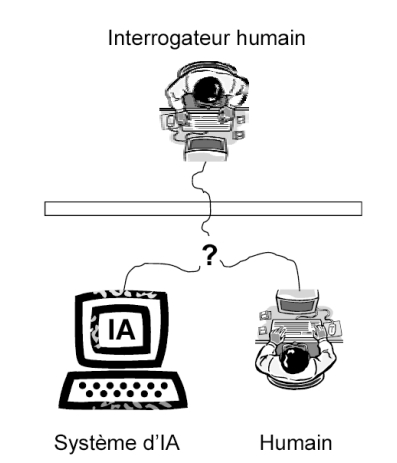
\includegraphics[width=10cm,height=6cm]{images/Test de turing.jpeg}%
    }
    \caption{Test de Turing.}%
\end{figure}

\subsection{Définition}
Selon \textbf{John McCarthy}, l’un des pionniers du domaine, l’IA est « la science et l’ingénierie de la fabrication de machines intelligentes ». C’est un domaine de l’informatique qui cherche à créer des systèmes capables de réaliser des tâches qui nécessiteraient normalement l’intelligence humaine.

Cependant, l’IA est souvent considérée comme un concept vaste et multidimensionnel, difficile à définir précisément en raison de sa nature étendue et en constante évolution.
\\
Elle est également définie par l'un de ses créateurs, \textbf{Marvin Lee Minsky}, comme « la construction de programmes informatiques qui s'adonnent à des tâches qui sont, pour l'instant, accomplies de façon plus satisfaisante par des êtres humains, car elles demandent des processus mentaux de haut niveau tels que : l'apprentissage perceptuel, l'organisation de la mémoire et le raisonnement critique » \cite{Lee}. On y trouve donc le côté « artificiel » atteint par l'usage des ordinateurs ou de processus électroniques élaborés et le côté « intelligence » associé à son but d'imiter le comportement.

\subsection{Classification de l’intelligence artificielle}

La classification de l’intelligence artificielle a pour vocation de permettre la compréhension des différentes catégories de systèmes développés dans ce domaine. Nous proposons ci-dessous les trois types d'IA :
\begin{itemize}  
	\item[\ding{118}]\textbf{L’IA faible}: également connue sous le nom d’IA étroite, elle désigne des systèmes d’IA spécialisés dans une tâche spécifique. Ces systèmes sont conçus pour effectuer une seule tâche de manière très performante, mais ils ne possèdent pas la capacité d’apprentissage ni la compréhension générale du contexte comme le font les humains. Ce qui démontre fort heureusement que l’humain a encore toute sa place dans les tâches et n’est pas prêt à être remplacé par l’IA.
	 
	\item[\ding{118}] \textbf{L’IA forte } : également connue sous le nom d’IA générale, représente un niveau supérieur d’intelligence artificielle. Contrairement à l’IA faible, l’IA forte possède la capacité d’apprendre par elle-même, de comprendre le contexte et de s’adapter à de nouvelles situations. Ainsi, bien que privée de conscience, qui reste quant à elle propre aux organismes vivants, la machine acquiert de l’expérience lui permettant de modifier son propre fonctionnement. Autrement dit, un apprentissage complémentaire découle des tâches qu’elle réalise, ce qui entraîne des réactions initialement non programmées. Ce niveau d’IA est encore largement théorique et n’a pas encore été pleinement atteint, bien que des progrès significatifs aient été réalisés dans le domaine de l’apprentissage automatique et des réseaux neuronaux.
	
	\item[\ding{118}] \textbf{La superintelligence artificielle} : le jour où l’IA dépassera l’intelligence humaine (notamment quand elle aura conscience de son existence) on parlera de superintelligence artificielle. On en est encore loin, mais avec les récentes évolutions très fortes et rapides dont l’humanité a été témoin (par exemple Chat GPT-4), il est légitime de penser que la superintelligence artificielle verra le jour dans le courant du 21e siècle. 
\end{itemize} 

\subsection{Domaines d'application}
L'IA a connu une évolution rapide ces dernières années et a pris une place prépondérante dans notre vie quotidienne. De plus en plus, nous voyons l'intégration de solutions d'IA dans divers aspects de notre vie pour améliorer notre quotidien. Cependant, l'IA est un domaine vaste, et il existe différents domaines d'application adaptés à des besoins spécifiques dans notre vie quotidienne. Dans cette section, nous explorerons ses principaux domaines d'application. 

\subsubsection{La robotique} La robotique a recours à l'IA à plusieurs égards. Notamment pour la perception de l'environnement (objets et visages), l'apprentissage et l'IA développementale. L'interaction homme-robot manque encore souvent de naturel et est un enjeu de la robotique. Il s'agit de permettre aux robots d'évoluer dans le monde dynamique et social des humains et d'échanger avec eux de façon satisfaisante. 

\subsubsection{Le militaire} Le domaine militaire utilise de plus en plus l'IA, notamment pour le pilotage automatique, le guidage de missiles, l'identification, le commandement, l'aide à la décision, la cyberguerre et la cyberdéfense, ou pour la documentation et les processus administratifs. À titre illustratif, confrontés à des missions à risques, les États-Unis se positionnent comme précurseurs de l’intelligence artificielle dans le secteur militaire. Leur production propose des robots autonomes ou télécommandés, pourvus d’une IA, permettant ainsi de remplacer l’Homme en position de combat.
 
\subsubsection{La médecine} Principalement importée de façon robotique, l’IA augmente la croissance de nombreux domaines liés à la technologie. La médecine en est un des exemples les plus concrets depuis 1980, date qui a signé l’apparition des premiers robots de guidage dans les blocs opératoires. Ces derniers permettent grâce à des capteurs de réaliser des mouvements miniaturisés dotés d’une grande précision. La médecine a aussi vu de grands progrès grâce à l'utilisation de systèmes d'aide au diagnostic ou de diagnostic automatisé. \\ C'est dans ce sens que Google DeepMind a également conçu AlphaFold, un système d'IA utilisant l'apprentissage profond qui permet de prédire la façon dont des protéines se replient. 

\subsubsection{Le droit} Le droit fait appel à l'IA dans la perspective de prédire les décisions de justice, d'aider à la décision et de trancher les cas simples. L'Estonie a par exemple développé une intelligence artificielle capable de prendre des décisions de justice sur des délits mineurs. Les États-Unis utilisent par ailleurs dans certaines juridictions le système COMPAS (Correctional Offender Management Profiling for Alternative Sanctions), un système d'aide à la prise de décision pour les juges. 

\subsubsection{Art et littérature} Les IA sont en mesure de produire des compositions musicales imitant le style du compositeur de notre choix. De même, certaines intelligences artificielles peuvent s’approprier le style d’écriture d’un écrivain célèbre et produire une œuvre littéraire qui pourrait très bien compter dans la bibliographie de l’auteur. D’ailleurs, en 2016, un prix littéraire a failli être décerné à une IA japonaise ayant coécrit une nouvelle.

\section{Les domaines de l'intelligence artificielle}
Les domaines de l’IA réside dans une base, qui fait référence aux éléments fondamentaux qui composent la technologie. Ces éléments de base comprennent, entre autres, l’apprentissage automatique, l'apprentissage profond, le traitement du langage naturel et la vision par ordinateur. Ensemble, ces composants forment l’épine dorsale de l’IA, permettant aux machines d’apprendre, de s’adapter et de s’améliorer au fil du temps.

\subsection{L'apprentissage automatique}
L'apprentissage automatique est un sous-ensemble de l'IA qui se concentre sur le développement d'algorithmes permettant aux machines d'apprendre à partir de données et de faire des prédictions ou des décisions sans être explicitement programmées. Par exemple, une plateforme de commerce électronique utilise des algorithmes d’apprentissage automatique pour recommander des produits aux clients en fonction de leur historique de navigation, de leurs achats et de leur historique de recherche. \\
Dans le chapitre suivant, nous verrons en long et en large ce qui est de l'apprentissage automatique.

\subsection{L'apprentissage profond}
L'apprentissage profond, également connu sous sa dénomination anglaise "Deep Learning" (DL), est en effet un cas particulier de l'apprentissage automatique. Il repose sur l'utilisation de réseaux de neurones artificiels, des structures algorithmiques inspirées du fonctionnement du cerveau humain. Ce type d'apprentissage est caractérisé par l'utilisation de 5 couches de neurones ou plus, permettant ainsi de capturer des représentations complexes des données en plusieurs niveaux d'abstraction.

\subsection{Le traitement du langage naturel}
Le traitement du langage naturel (NLP) fait référence à la capacité des machines à comprendre, interpréter et générer le langage humain. La NLP est essentielle pour les chatbots, les assistants virtuels et les systèmes de reconnaissance vocale qui permettent aux utilisateurs d'interagir avec les machines en utilisant le langage naturel.

\subsection{La vision par ordinateur}
La vision par ordinateur implique d’entraîner des machines à interpréter et à comprendre les données visuelles du monde qui les entoure. Grâce à la vision par ordinateur, les machines peuvent reconnaître des objets, des visages et même des émotions, ce qui est essentiel pour des applications telles que la reconnaissance faciale, la surveillance et les voitures autonomes.

\begin{figure}[H]%
    \center%
    \setlength{\fboxsep}{5pt}%
    \setlength{\fboxrule}{0.5pt}%
    \fbox{
    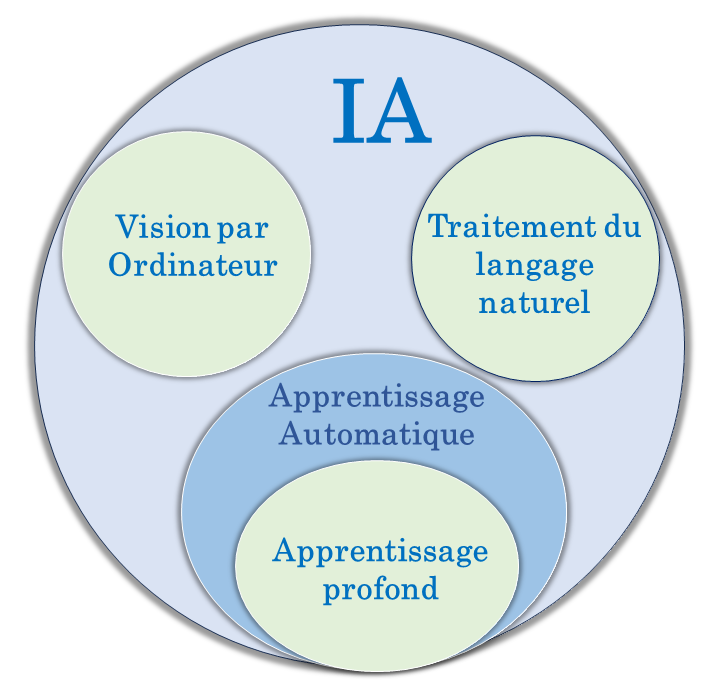
\includegraphics[width=8cm,height=6cm]{images/fondemdent de IA.png}%
    }
    \caption{Fondement de IA.}%
\end{figure}

\section{L'avenir de l'IA et son impact potentiel}
L'IA façonne l'avenir de la technologie et révolutionne notre façon de vivre, de travailler et de communiquer. Les progrès réalisés dans le domaine de l’IA ont transformé la façon dont nous interagissons avec la technologie et les machines, et les possibilités de ce que l’IA peut réaliser sont infinies. Cependant, le potentiel de l’IA s’accompagne également de risques et de défis potentiels qui doivent être surmontés\cite{fastercapital}. Dans cette section, nous discuterons de l’avenir de l’IA et de son impact potentiel sur la société.

\subsection{Le progrès de l’IA }
Les progrès réalisés dans le domaine de l’IA ont été remarquables et la technologie a parcouru un long chemin ces dernières années. Les machines basées sur l’IA peuvent désormais apprendre et s’adapter à de nouvelles situations, effectuer des tâches complexes et même prendre des décisions par elles-mêmes. Les applications potentielles de l’IA sont vastes, depuis les voitures autonomes jusqu’aux soins de santé personnalisés.

\subsection{L'impact sur le marché du travail}
L'essor de l'IA a suscité des inquiétudes quant à son impact sur le marché du travail. Les machines basées sur l’IA peuvent effectuer des tâches qui étaient autrefois effectuées par des humains, ce qui pourrait entraîner des suppressions d’emplois. Cependant, de nombreux experts affirment que l’IA créera de nouveaux emplois et opportunités, et que les humains seront toujours nécessaires pour superviser et entretenir les machines alimentées par l’IA.

\subsection{Les préoccupations éthiques}
L’utilisation de l’IA soulève également des préoccupations éthiques, notamment en ce qui concerne les questions de confidentialité et de préjugés. Par exemple, les systèmes basés sur l’IA qui utilisent la technologie de reconnaissance faciale pourraient être utilisés pour envahir la vie privée des gens. Il existe également des inquiétudes quant aux préjugés dans les systèmes d’IA, car ils peuvent perpétuer les préjugés et la discrimination existants.

\subsection{Le potentiel du bien}
Malgré les risques et les défis potentiels, l’IA a le potentiel de faire beaucoup de bien. Les machines basées sur l'IA peuvent nous aider à relever certains des plus grands défis mondiaux, du changement climatique aux soins de santé. Par exemple, les capteurs basés sur l’IA peuvent être utilisés pour surveiller et réduire les émissions de carbone, tandis que les systèmes de santé basés sur l’IA peuvent aider les médecins à diagnostiquer et à traiter les maladies avec plus de précision et d’efficacité.

\section{Conclusion}
Ce premier chapitre nous a offert une exploration complète de l'intelligence artificielle, depuis ses origines historiques jusqu'à son domaine d'application actuel. Il nous a permis de comprendre ces 4 fondements qui constituent l'épine dorsale de l'IA, permettant aux machines d'apprendre, de s'adapter et de s'améliorer au fil du temps, et nous avons pu examiner l'avenir de l'IA et son impact potentiel.


    \chapter{GÉNÉRALITÉ SUR LE MACHINE LEARNING}
\begin{spacing}{1.2}
\minitoc
\thispagestyle{MyStyle}
\end{spacing}
\newpage

Le machine learning, abrégé ML, représente l’une des branches les plus captivantes de l’intelligence artificielle, un sujet qui pourrait remplir un livre entier à lui seul. Cette approche technologique révolutionnaire permet aux experts en données, communément appelés « Data Scientists », d’alimenter les algorithmes avec des ensembles de données, donnant ainsi aux machines la capacité d’apprendre et de prendre des décisions sans nécessiter de programmation informatique préalable.
\\
Dans ce chapitre, nous commencerons par une présentation du machine learning (ML), nous aborderons ensuite la classification des méthodes et les algorithmes de ML, et nous découvrirons enfin à travers ce chapitre les étapes du processus du ML.

\section{Présentation de machine leaning}

\subsection{Contexte}
Nous générons toujours plus de données chaque jour avec la multiplicité des technologies que nous utilisons 
(smartphones, ordinateurs, tablettes, objets connectés…). Tous ces appareils génèrent une quantité de données massive. Une personne génère en moyenne 1,7 Mo de 
données par seconde en 2020. L’ensemble de ces données est stocké en bases numériques et représente une source d’informations considérable : c’est le Big Data \cite{Azencott_chloe}. 
Mais sans traitement adéquat ni stratégie d’analyse efficace, cette masse de données ne resterait qu’un amas d’octets problématiques à entasser. C’est à ce moment 
que le Machine Learning intervient et permet de tirer profit de ces données.

\subsection{Définition}
L'apprentissage automatique, un sous-ensemble de l'intelligence artificielle, donne aux ordinateurs la capacité d'apprendre et de faire des prédictions ou des décisions basées sur des données. Cela implique le développement d’algorithmes capables d’apprendre et de s’améliorer automatiquement à partir de l’expérience sans être explicitement programmés. 

\subsection{Rôle de machine learning dans l'intelligence artificielle}
Le machine learning est crucial pour IA car il permet aux systèmes d'apprendre et de s'améliorer à partir de données, sans intervention humaine. Cette capacité d'adaptation rend les systèmes d'IA plus précis et efficaces, en particulier dans des tâches complexes comme la reconnaissance d'images et la compréhension du langage naturel. De plus, le machine learning est au cœur de nombreuses applications pratiques, de la recommandation de produits à la détection de fraudes. Il permet également l'automatisation de tâches, réduisant les coûts et augmentant l'efficacité. En constante évolution, le machine learning favorise l'innovation continue et la personnalisation des expériences utilisateur, transformant ainsi divers secteurs et améliorant la qualité de nombreux services.

\section{Fonctionnement de machine learning}
Le ML fonctionne en suivant un processus général composé de quatre étapes principales : la collecte de données, le prétraitement des données, la formation du modèle et l'évaluation du modèle \cite{fastercapital_ml}.

\subsection{Collecte de données}
La collecte de données est la première et la plus importante étape de l'apprentissage automatique, où les données pertinentes et suffisantes sont collectées à partir de diverses sources, telles que des bases de données, des pages Web, des capteurs, des enquêtes, etc. La qualité et la quantité des données déterminent les performances et la précision du modèle d'apprentissage automatique. Il est donc essentiel de collecter des données représentatives, diverses et impartiales.

\subsection{Prétraitement des données}
Le prétraitement des données est la deuxième étape du ML, où les données brutes sont nettoyées, transformées et préparées pour le modèle. Le prétraitement des données implique des tâches telles que la gestion des valeurs manquantes, des valeurs aberrantes et du bruit, le codage des variables catégorielles, la mise en échelle des variables numériques, l'ingénierie des fonctionnalités, la sélection des fonctionnalités et le fractionnement des données.\\ 
Le prétraitement des données vise à améliorer la qualité et la convivialité des données et à réduire la complexité et la dimensionnalité des données.

\subsection{Entraînement de modèle}
L'entraînement de modèle est la troisième étape du ML, où le modèle est construit et formé sur les données pré-traitées. Il implique de choisir un algorithme d'apprentissage automatique approprié, tel qu'un arbre de décision, un réseau de neurones, une machine à vecteurs de support, etc., et d'ajuster ses paramètres, tels que le taux d'apprentissage, le nombre d'itérations, le terme de régularisation, etc.\\ 
L'entraînement sur modèle vise à trouver les paramètres optimaux qui minimisent la fonction d’erreur ou de perte et maximisent la précision ou la mesure de performance.

\subsection{Évaluation du modèle}
L'évaluation du modèle est la quatrième et dernière étape du ML, où le modèle est testé et validé sur des données invisibles. L'évaluation du modèle consiste à mesurer la capacité de généralisation et la robustesse du modèle d'apprentissage automatique, à l'aide de mesures telles que l'exactitude, la précision, le rappel, le score f1, la courbe d'évaluation, etc. \\ 
Elle vise à évaluer l'efficacité et la fiabilité du modèle d'apprentissage automatique et à identifier les domaines d'amélioration ou de modification.
\begin{figure}[H]%
    \center%
    \setlength{\fboxsep}{5pt}%
    \setlength{\fboxrule}{0.5pt}%
    \fbox{
    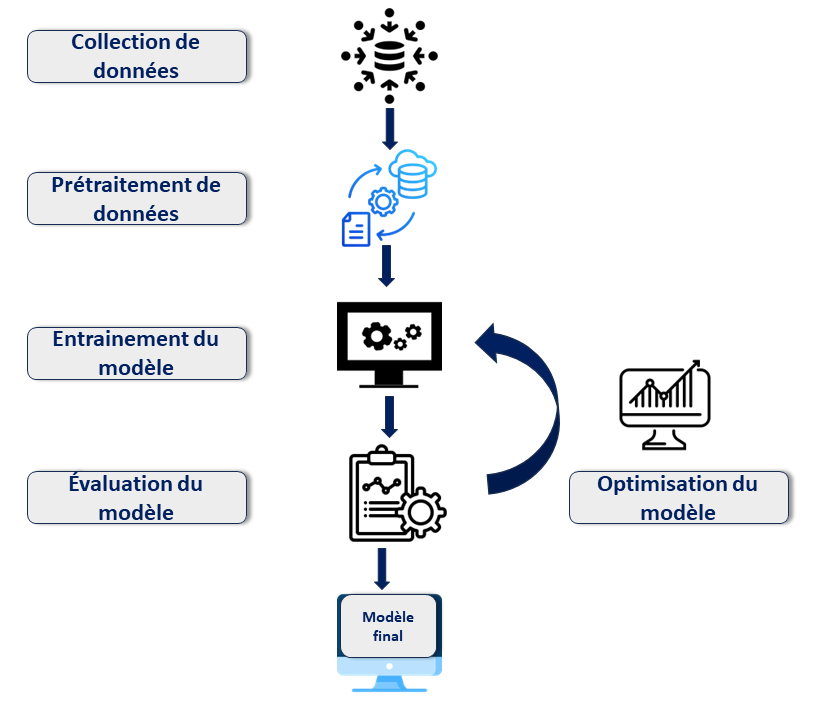
\includegraphics[width=10cm,height=6cm]{images/fonctionnement de ml.png}%
    }
    \caption{Fonctionnement de ML.}%
\end{figure}

\section{Classification des approches de machine learning et leurs algorithmes}

Les approches et algorithmes d'apprentissage automatique sont les moteurs des progrès de l'intelligence artificielle et de l'analyse des données. Ces approches et algorithmes permettent aux machines d'apprendre des données et de faire des prédictions ou des décisions sans programmation explicite. En analysant de grands ensembles de données et en identifiant les modèles, les algorithmes d'apprentissage automatique peuvent découvrir des informations cachées et fournir des prédictions précieuses pour diverses industries et applications.

Il existe plusieurs types d'approches et d'algorithmes d'apprentissage automatique, chacun conçu pour résoudre différents types de problèmes. Dans cette partie, nous allons explorer certaines des principales approches et algorithmes les plus couramment utilisés et leurs applications.

\subsection{Apprentissage supervisé}
L'apprentissage supervisé consiste à entraîner des modèles sur des ensembles de données étiquetés, où chaque point de données est associé à une valeur de résultat ou de cible connue \cite{mohri2012}. Ces modèles apprennent à partir de ces données étiquetées et sont capables de faire des prédictions sur des données inconnues ou futures. 
\begin{figure}[H]%
    \center%
    \setlength{\fboxsep}{5pt}%
    \setlength{\fboxrule}{0.5pt}%
    \fbox{
    \includegraphics[width=10cm,height=6cm]{images/apprentissage supervisé.png}%
    }
    \caption{Apprentissage supervisé.}%
\end{figure}
Fondamentalement, le ML supervisé revient à apprendre à une machine à construire une fonction \( f \) telle que \( Y = f(X) \), \( Y \) étant un ou plusieurs résultats d'intérêt calculés en fonction des données d'entrée \( X \) effectivement à la disposition de l'utilisateur. \( Y \) peut être une grandeur continue (une température par exemple), et on parle alors de régression, ou discrète (une classe, chien ou chat par exemple), et on parle alors de classification. L'apprentissage supervisé est donc divisé en deux catégories principales : la classification et la régression.

\subsubsection{Les algorithmes de classification}
La classification automatique, également connue sous le nom de classification supervisée, est une méthode algorithmique qui consiste à attribuer des classes ou des catégories discrètes à des objets en fonction de caractéristiques ou de variables d'entrée. L'objectif est de construire un modèle qui puisse prédire la classe correcte pour de nouveaux exemples basés sur des exemples préalablement étiquetés dans l'ensemble de données d'apprentissage. Les algorithmes de classification sont largement utilisés dans divers domaines tels que la reconnaissance de texte, la détection de spam, la classification d'images et bien d'autres.

Différents algorithmes de classification existent, chacun avec ses propres caractéristiques et fonctionnalités. Certains des algorithmes de classification les plus couramment utilisés comprennent : \textbf{Arbres de décision}, \textbf{Machine à Vecteur de support (SVM)}, \textbf{K plus proches voisins (KNN)}, \textbf{Réseaux de neurones artificiels}, etc.

\subsubsection{Les algorithmes de régression}
Contrairement à la classification qui prédit une catégorie ou une étiquette, les modèles de régression prédisent une valeur de sortie continue, en fonction de la variable indépendante d’entrée. Cette technique est utilisée lorsque la variable de sortie à prédire doit être une valeur continue, soit par exemple pour les prédictions météorologiques ou pour les tendances de marché. Différents modèles de régression existent et diffèrent dépendant de la relation entre la variable dépendante et indépendante considérée, ainsi que du nombre de variables indépendantes utilisées pour le modèle. Parmi les principaux modèles de régression : \textbf{Régression logistique binaire}, \textbf{Régression logistique multiclasse}, \textbf{Régression linéaire simple}, \textbf{Régression linéaire multiple}, \textbf{Régression à vecteurs de support (RVM)}, etc.

\subsection{Apprentissage non supervisé}
L'apprentissage non supervisé est un sous-champ d'apprentissage automatique qui se concentre sur l'identification des modèles et des relations cachés dans les données sans utiliser d'exemples étiquetés ou pré-classifiés \cite{sublime2022}. Contrairement à l'apprentissage supervisé, qui consiste à former un modèle sur un ensemble de données étiqueté et à l'utiliser pour faire des prédictions sur de nouvelles données invisibles, des algorithmes d'apprentissage non supervisés fonctionnent sur des données brutes et non marquées et visent à découvrir les structures ou les relations sous-adjacentes. L'algorithme doit découvrir par lui-même la structure plus ou moins cachée des données.
\begin{figure}[H]%
    \center%
    \setlength{\fboxsep}{5pt}%
    \setlength{\fboxrule}{0.5pt}%
    \fbox{
    \includegraphics[width=12cm,height=6cm]{images/apprentissage non-supervisé.png}%
    }
    \caption{Apprentissage non supervisés.}%
\end{figure}

Fondamentalement, le machine learning non supervisé revient à apprendre à une machine à construire une fonction \( f \) telle que \( Y = f(X) \), \( Y \) étant un ou plusieurs résultats d'intérêt calculés en fonction des données d'entrée \( X \) effectivement à la disposition de l'utilisateur. \( Y \) peut être une grandeur continue (par exemple, une caractéristique mesurée), et on parle alors de réduction de dimensionnalité ou de clustering, ou discrète (par exemple, un groupe ou une catégorie), et on parle alors de segmentation ou de classification automatique. L'apprentissage non supervisé est donc un processus visant à découvrir des structures ou des groupes naturels dans les données, sans qu'il soit nécessaire de fournir des exemples étiquetés.

\subsubsection{Les algorithmes de partitionnement ou le Clustering}
Les algorithmes de partitionnement sont des techniques d'apprentissage non supervisé qui visent à diviser un ensemble de données en plusieurs clusters ou groupes, où chaque cluster est une collection de points de données similaires. L'objectif est de partitionner les données de manière à ce que les points à l'intérieur de chaque cluster soient similaires les uns aux autres, tandis que les points de différents clusters soient différents. Parmi ceux-ci figurent: \textbf{k-means}, \textbf{Clustering hiérarchique}, \textbf{Mean Shift}, \textbf{DBSCAN}, etc.

\subsubsection{Les algorithmes de la réduction de la dimensionnalité}
La réduction de la dimensionnalité vise à réduire le nombre de variables aléatoires dans un ensemble de données, tout en préservant autant que possible les caractéristiques importantes des données. Cela est souvent nécessaire lorsque les données sont très complexes et comprennent un grand nombre de dimensions, ce qui peut rendre l'analyse et la visualisation difficiles. Il est couramment utilisé dans l'étape de pré-traitement des données, et il existe différents algorithmes de réduction de la dimensionnalité qui peuvent être utilisés, à savoir : \textbf{Auto-encodeurs}, \textbf{Décomposition en valeurs singulières (DVS)}, \textbf{Principal Component Analysis}, \textbf{Locally Linear}, etc.

\subsection{Apprentissage par renforcement}
L'apprentissage par renforcement ou le Reinforcement Learning (RL) en anglais est un sous-ensemble de l'apprentissage automatique qui permet à un système piloté par l'IA (parfois appelé un agent) d'apprendre par tâtonnements à l'aide d'un retour d'information à partir de ses actions. Cette rétroaction est soit négative soit positive, qualifiée de punition ou de récompense avec, bien sûr, l'objectif de maximiser la fonction de récompense. RL apprend de ses erreurs et offre une intelligence artificielle qui imite l'intelligence naturelle aussi étroitement que possible.

En termes de méthodes d'apprentissage, RL est similaire à l'apprentissage supervisé uniquement en ce qu'il utilise la cartographie entre l'entrée et la sortie, mais c'est la seule chose qu'ils ont en commun. Alors que dans l'apprentissage supervisé, le retour d'information contient l'ensemble correct d'actions à prendre par l'agent. Dans le RL, il n'existe pas de clé de réponse de ce type. L'agent décide de ce qu'il faut faire lui-même pour effectuer la tâche correctement. Comparé à l'apprentissage non supervisé, le RL a des objectifs différents. L'objectif de l'apprentissage non supervisé est de trouver des similitudes ou des différences entre les points de données. L'objectif de RL est de trouver le modèle d'action le plus approprié pour maximiser la récompense cumulée totale pour l'agent RL. En l'absence d'ensemble de données de formation, le problème RL est résolu par les propres actions de l'agent avec l'apport de l'environnement.
De nombreux algorithmes d'apprentissage de renforcement utilisent des techniques de programmation dynamique \cite{vanotterlo2012}.
L'environnement dans un algorithme d'apprentissage de renforcement est généralement exprimé sous la forme d'un processus de décision de Markov (MDP), et presque tous les problèmes de RL sont formalisés à l'aide de MDP.\\
Dans l'apprentissage par renforcement, nous devons nous familiariser avec quelques concepts clés :
\begin{itemize}
	\item[\ding{118}] \textbf{L'agent} : qui est l'algorithme de ML (ou le système autonome).
	\item[\ding{118}] \textbf{L'environnement} : qui est l'espace adaptatif du problème avec des attributs tels que des variables, des valeurs limites, des règles et des actions valides.
	\item[\ding{118}] \textbf{L'action} : qui est une étape que l'agent de RL effectue pour naviguer dans l'environnement.
	\item[\ding{118}] \textbf{L'état} : qui est l'environnement à un moment donné.
	\item[\ding{118}] \textbf{La récompense} : qui est la valeur positive, négative ou nulle pour avoir effectué une action, en d'autres termes, la récompense ou la punition.
	\item[\ding{118}] \textbf{La politique} : qui est une stratégie que l'agent suit pour sélectionner une action dans chaque état.
	
\end{itemize}
\begin{figure}[H]%
    \center%
    \setlength{\fboxsep}{5pt}%
    \setlength{\fboxrule}{0.5pt}%
    \fbox{
    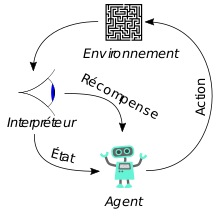
\includegraphics[width=8cm,height=6cm]{images/Reinforcement_learning_diagram_fr.svg.png}%
    }
    \caption{Apprentissage par renforcement.}%
\end{figure}
Dans le RL, de nombreux algorithmes sont utilisés tels que Q-Learning, Policy Gradient Methods, SARSA (State-Action-Reward-State-Action), Monte Carlo Methods, Temporal Difference Learning, etc. Tous ces algorithmes peuvent être regroupés en deux grandes catégories.
 
\subsubsection{Apprentissage par renforcement Axé sur un Modèle (Model-Based RL)}
Dans cette approche, l’agent construit un modèle interne de l’environnement. Ce modèle
peut être utilisé pour simuler les transitions d’états et les récompenses, ce qui permet à l’agent de
planifier ses actions avant de les exécuter dans l’environnement réel. Les algorithmes de RL axés
sur un modèle comprennent les méthodes de Monte Carlo avec modèle et certaines variantes
de l’apprentissage par différence temporelle. Parmi ces algorithmes figurent : \textbf{Model-Based
Actor-Critic}, \textbf{Dyna-Q}, \textbf{Dynammic Programming}, \textbf{Model Predictive Control} , etc.

\subsubsection{Apprentissage par renforcement sans Modèle (Model-Free RL)}
Dans cette approche, l'agent n'apprend pas explicitement un modèle de l'environnement, mais apprend plutôt à partir d'expériences directes dans l'environnement. L'agent utilise des interactions réelles avec l'environnement pour estimer la valeur des états ou des actions et pour apprendre une politique optimale sans avoir besoin de connaître les transitions d'états ou les récompenses à l'avance. Les algorithmes de RL sans modèle comprennent le Q-Learning, les méthodes de gradients de politique et certains types d'apprentissage par différence temporelle. ce sont: \textbf{Q-Learning}, \textbf{SARSA}, \textbf{Deep Q-Networks}, \textbf{Temporal Difference Learning} 

\section{Conclusion}
Ce deuxième chapitre a offert une introduction complète au machine learning, définissant
ses principes fondamentaux et soulignant son rôle central dans l’IA. Il a également décomposé
le processus du machine learning en étapes clés, de la collecte des données à l’évaluation des
modèles, tout en survolant les principales approches du machine learning, notamment l’apprentissage
supervisé, non supervisé et par renforcement, offrant ainsi un aperçu des algorithmes associés.
    
    \chapter{APPROCHE MÉTHODIQUE ET MODÉLISATION}
\begin{spacing}{1.2}
\minitoc
\thispagestyle{MyStyle}
\end{spacing}
\newpage

L’évaluation de la réussite des étudiants est une préoccupation majeure dans le domaine de l’enseignement. L'utilisation de l'intelligence artificielle, en particulier l'apprentissage automatique, s'est révélée être un outil puissant pour aborder ce défi. De nombreuses études ont exploré l'application de techniques d'apprentissage automatique dans la prédiction des performances académiques des étudiants, cherchant à identifier les facteurs clés qui influencent le succès universitaire. \\
C'est dans cette perspective que ce chapitre consistera à aborder l'état de l'art sur la prédiction de réussite des étudiants, une approche de solution, et la modélisation de notre solution pour prédire la réussite en licence économie à l'UNZ en utilisant l'intelligence artificielle.

\section{État de l'art}
De nombreuses études ont été menées pour prédire avec précision la réussite des étudiants, afin de mettre en place des mesures d'intervention précoce et d'améliorer les politiques éducatives. L'utilisation de l’intelligence artificielle dans ce domaine a produit des résultats prometteurs. Cette section passe en revue les principales études antérieures sur la prédiction des réussites des étudiants, mettant en évidence les méthodes et techniques utilisées, ainsi que les défis et limitations rencontrés.

\subsection{Études antérieures sur la prédiction des réussites des étudiants}
La prédiction de la réussite des étudiants a été abordée par de nombreuses études à travers le monde. Ces études ont généralement utilisé une variété de techniques, allant des modèles statistiques traditionnels aux approches plus récentes basées sur l'apprentissage automatique et l'intelligence artificielle. Parmi les études les plus remarquables, celles-ci se sont concentrées sur l'utilisation de données démographiques des étudiants, telles que le sexe, l'âge et le niveau socio-économique, ainsi que sur les performances académiques antérieures, telles que les notes et les résultats aux examens standardisés.

Dans une étude menée par \textbf{Jean-Philippe Vandamme}, \textbf{Nadine Meskens} et \textbf{Abdelhakim Artiba}, l'échec scolaire en première année universitaire a été le sujet central de recherche \cite{vandamme2023comparison}. Cette problématique a suscité de nombreux débats parmi les psychopédagogues qui ont cherché à la comprendre et à l'expliquer, tandis que les statisticiens se sont attelés à le prévoir.
L'objectif de leurs recherches était de développer un modèle permettant de déterminer, dès le début de l'année universitaire, le groupe d'étudiants de première année qui nécessitait prioritairement des ressources pédagogiques pour améliorer leur taux de réussite. Pour ce faire, ils ont élaboré un questionnaire basé sur les hypothèses posées dans de nombreux modèles théoriques, puis ils ont collecté des données diverses et nombreuses à l'aide de ce questionnaire.
Ensuite, à l'aide de méthodes statistiques ou de fouille de données (data mining\textsuperscript{} \footnote{\textbf{Data mining} est l'analyse de données volumineuses pour trouver des corrélations, des patterns et du savoir.}), leur objectif était d'extraire des informations permettant de classer les étudiants en trois classes les plus homogènes possible.
La mise en parallèle des résultats fournis par les différentes méthodes, telles que les analyses discriminantes, les régressions, les ensembles approximatifs et les arbres de décision, a permis de mettre en lumière leurs différences de performance. En effet, certaines méthodes se sont avérées plus efficaces en termes de taux de prédictions correctes réalisées, tandis que d'autres ont été plus intéressantes pour leur capacité à identifier les facteurs prédictifs de la réussite universitaire.

\textbf{Kanduki Kivuyirwa Mystère}, \textbf{Héritier Nsenge Mpia} et \textbf{Mutegheki Baraka Vingi} ont aussi étudié la prédiction de l'orientation des étudiants dans des filières d’études appropriées en utilisant les techniques de Data Mining \cite{mystere2023prediction}. Leur étude met en lumière l'utilisation de nombreuses techniques de Data Mining pour extraire des connaissances cachées dans des données éducatives, dans le but d'aider les étudiants à prendre des décisions utiles pour leur orientation à l’université.
Cette recherche, basée sur un questionnaire d'enquête ayant recueilli 712 réponses, a permis aux auteurs de réaliser l'entraînement de modèles de prédiction. Les performances de ces modèles ont ensuite été évaluées à l'aide de mesures telles que l'accuracy \textsuperscript{} \footnote{\textbf{Accuracy} est l’exactitude représentant la justesse globale des prédictions d’un modèle.}, la précision, le recall \textsuperscript{} \footnote{\textbf{Recall} est une métrique qui permet de mesurer la capacité d’un modèle à retrouver les exemples positifs réels dans un ensemble de données.} et le F-score\textsuperscript{} \footnote{\textbf{F-score} est une métrique utilisée pour évaluer la précision et les performances des modèles de classification.}. Les résultats ont montré que l'algorithme SVM a obtenu le meilleur score avec 70\% d’accuracy, suivi par le Naïve Bayes avec 65\% d’accuracy, le Réseau de neurones avec 64\%, tandis que l’arbre de décision n'a donné que 52\% d’accuracy. Ces résultats ont conduit les chercheurs à sélectionner le SVM comme le modèle le plus performant.

En complément des recherches précédentes, une étude significative menée par \textbf{Moustapha Bikienga}, \textbf{Ozias Bombiri} et \textbf{Emmanuel Sawadogo} a porté sur la conception d'un modèle basé sur l'apprentissage automatique pour la prédiction des performances académiques \cite{bikienga2023design}. Leurs recherchent s'inscrivent dans le cadre de l'amélioration des systèmes d'orientation des étudiants en utilisant des modèles prédictifs.
Dans leur étude, les chercheurs ont mis en évidence l'importance de prédire et d'analyser les performances des étudiants afin de concevoir des processus d'orientation utiles, permettant d'obtenir des taux de réussite élevés et d'améliorer le classement de l'institution en tant que critère de qualité d'une université. Ils soulignent également que le manque de soutien adéquat et d'orientation personnalisée accroît le taux d'échec des étudiants.
Pour évaluer la possibilité d'améliorer le système d'orientation des étudiants, les chercheurs ont développé un modèle basé sur l'apprentissage automatique dans le but de prédire les chances de succès des étudiants de l'UFR-ST de l'UNZ. Ils ont utilisé plusieurs algorithmes d'apprentissage automatique (Adaboost, Random Forest, SVM et KNN) pour ajuster le modèle avec les données de réalisations des étudiants des années académiques 2017-2018 et 2018-2019.
Les résultats obtenus sur les données de test ont révélé un score supérieur à 70\% pour le meilleur algorithme (Random Forest), démontrant ainsi l'efficacité de l'approche basée sur l'apprentissage automatique dans la prédiction des performances académiques des étudiants.

Une autre étude d'importance, menée par \textbf{Ozias Bombiri}, \textbf{Tounwendyam F. Ouédraogo}, \textbf{Paonouor Some} et \textbf{Pasteur Poda}, s'est centrée sur le développement d'un système d'orientation intelligent dans CAMPUSFASO\textsuperscript{} \footnote{\textbf{CAMPUSFASO} est la plateforme unique de gestion des procédures et d’orientation pour les nouveaux bacheliers burkinabè ou étrangers.} \cite{bombiri2022towards}. Cette recherche met en lumière l'importance de l'orientation, un domaine complexe et multidisciplinaire visant à aider les étudiants à trouver leur voie de formation adaptée. Depuis 2018, le système d'orientation universitaire a évolué avec la mise en place d'une plateforme en ligne appelée CAMPUSFASO. Cette plateforme, présentée comme une innovation dans le domaine de l'orientation, a néanmoins été fortement critiquée.
Dans leur étude, ils ont d'abord présenté les réalisations académiques des étudiants de première année de l'UNZ après avoir été orientés par CAMPUSFASO. Ces résultats ont montré que plus l'étudiant est guidé vers son parcours de formation préférentiel, plus il réussit académiquement.
Ensuite, ils proposent un modèle d'apprentissage automatique pour l'orientation. Contrairement à CAMPUSFASO, leur modèle utilise les notes de lycée de l'étudiant pour trouver le parcours de formation adapté. Ce modèle a obtenu des résultats satisfaisants avec des données simulées, démontrant ainsi son potentiel dans l'amélioration du système d'orientation des étudiants.

\subsection{Méthodes et techniques utilisées dans les recherches similaires}
Les méthodes et techniques utilisées dans les recherches sur la prédiction de la réussite des étudiants varient en fonction des données disponibles et des objectifs spécifiques de chaque étude. Certaines études ont utilisé des modèles de régression linéaire pour prédire les performances académiques des étudiants en se basant sur des données démographiques et des performances antérieures. D'autres ont opté pour des approches plus sophistiquées, telles que les réseaux neuronaux artificiels et les algorithmes d'apprentissage automatique, pour modéliser des relations complexes entre les caractéristiques des étudiants et leur réussite académique.

\subsection{Limitations et lacunes dans les approches existantes}
Bien que les études antérieures aient apporté des contributions importantes à la prédiction de la réussite des étudiants, elles présentent également certaines limites et lacunes. Parmi les principales limitations, on peut citer la dépendance excessive à l'égard des données démographiques et des performances antérieures, qui peuvent ne pas capturer tous les facteurs pertinents pour prédire la réussite des étudiants. De plus, certaines études ont été confrontées à des problèmes de généralisabilité, car les modèles développés dans un contexte particulier peuvent ne pas être applicables à d'autres contextes ou populations d'étudiants.

\section{Proposition de solution} 
Dans cette section, nous détaillerons notre solution proposée pour prédire la réussite en licence économie des étudiants orientés. Nous commencerons par une description générale de notre approche proposée, suivie du choix des données et des caractéristiques pertinentes que nous avons identifiées comme étant cruciaux pour notre modèle de prédiction. Enfin, nous discuterons des méthodes de prétraitement des données que nous avons employées pour garantir la qualité et la fiabilité de nos prédictions.

\subsection{Description générale de l'approche proposée}
Notre approche repose sur l'utilisation de l'intelligence artificielle, plus précisément l'apprentissage automatique, pour construire un modèle de prédiction de la réussite des étudiants sans tenir compte du type de licence. Nous collectons et utilisons diverses données. En utilisant ces données, nous cherchons à développer un modèle capable de prédire avec précision la probabilité de réussite des étudiants à leur licence en économie.

Il convient de noter que la licence économie comprend trois types de licences : Économie Agricole et de l'Environnement (EAE), Économie et sciences de gestion (ESG), et Analyse et Politique Économique (APE). Cependant, notre modèle ne précise pas le type de licence que l'étudiant réussira ou non. De plus, le modèle se base uniquement sur les notes de la première année pour prédire la réussite.
Dans notre approche, nous définissons qu'un étudiant a réussi s'il termine sa licence en économie dans le délai prévu par les textes de l'université (trois années académiques), c'est-à-dire qu'il n'a pas redoublé une année au cours de son parcours universitaire. Ainsi, un étudiant est considéré comme ayant réussi s'il obtient sa licence dans les trois années suivant son inscription initiale, sans avoir été contraint de redoubler une année académique. Cette définition de la réussite nous permet d'évaluer la performance des étudiants sur une période de temps définie et de déterminer si notre modèle de prédiction parvient à identifier avec précision les étudiants susceptibles de terminer leur licence dans les délais impartis.

\begin{figure}[H]%
    \center%
    \setlength{\fboxsep}{5pt}%
    \setlength{\fboxrule}{0.5pt}%
    \fbox{
    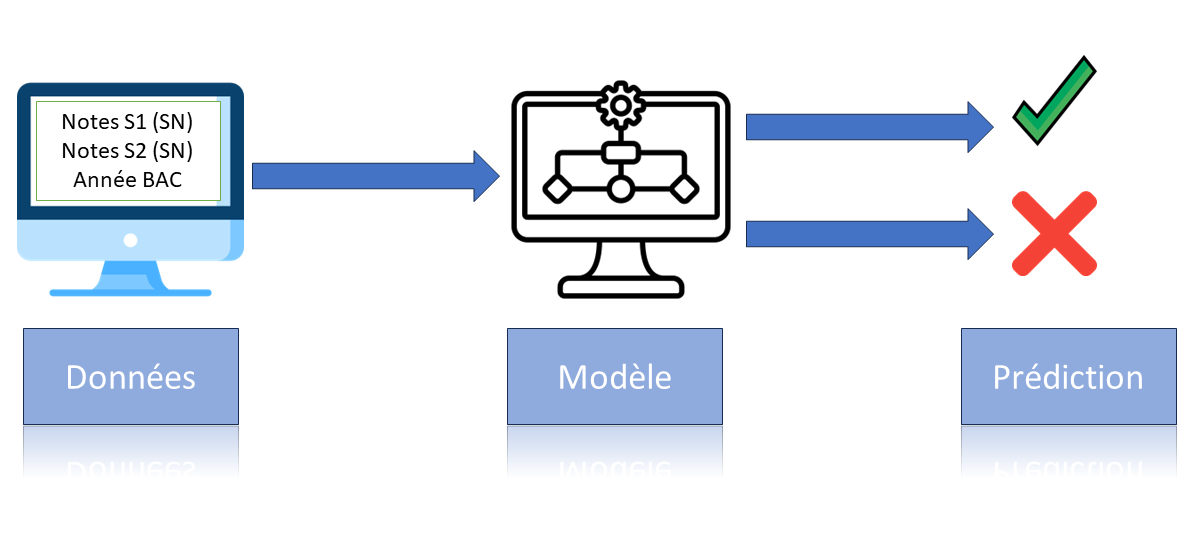
\includegraphics[width=10cm,height=6cm]{images/approce de solution.png}%
    }
    \caption{Approche de solution.}%
\end{figure}

\subsection{Choix des données et des caractéristiques pertinentes}
Pour notre modèle de prédiction, nous avons sélectionné un ensemble de données comprenant les notes des étudiants dans les matières clés du programme de licence économie, les années du baccalauréat, ainsi que d'autres caractéristiques pertinentes. Nous pensons que ces caractéristiques peuvent jouer un rôle important dans la prédiction de la réussite des étudiants en licence économie, en nous permettant de capturer à la fois les aspects académiques et non académiques qui peuvent influencer les performances des étudiants.

\subsection{Résultats attendus}
Les résultats que nous espérons obtenir de notre modèle de prédiction de la réussite des étudiants en licence économie sont basés sur nos objectifs initiaux.

Nous nous attendons à ce que notre modèle soit capable de prédire avec une précision élevée la probabilité de réussite des étudiants en licence économie. Nous visons une précision minimale de 70\% sur notre ensemble de données de test, ce qui signifie que le modèle doit être capable de classer correctement au moins 70\% des étudiants dans la bonne catégorie (réussite ou échec).

Nous attendons également d'évaluer les performances de notre modèle en mettant l'accent sur sa capacité à prédire de manière précise la réussite des étudiants indépendamment du type de licence.

Enfin, nous attendons d'analyser les facteurs prédictifs de la réussite des étudiants en licence économie, en identifiant les caractéristiques les plus importantes pour prédire leur réussite. Cela nous permettra de mieux comprendre les déterminants du succès des étudiants et de fournir des recommandations pour améliorer les taux de réussite.

\section{Modélisation}

\subsection{Choix du modèle}
Le choix du modèle de prédiction repose sur plusieurs critères, notamment la nature des données disponibles, la complexité du problème et les performances attendues. Dans notre étude, nous avons opté pour un modèle d'apprentissage supervisé en raison de la disponibilité de données étiquetées sur les réussites des étudiants en licence économie. Plus précisément, nous avons choisi d'utiliser des algorithmes de classification, car notre objectif est de prédire la probabilité de réussite des étudiants en les classant dans différentes catégories (réussite ou échec).

\subsection{Analyse et méthodes de prétraitement des données}
Avant d'entamer le processus d'entraînement de notre modèle de prédiction, une analyse approfondie de nos données s'est imposée.
L'analyse de la forme de nos données révèle un ensemble de 5655 étudiants et 31 colonnes. Parmi ces colonnes, 25 sont de type réel, 4 sont de type entier, et 3 sont de type objet ou chaîne de caractères, comprenant des informations telles que le nom, le prénom et le matricule des étudiants. 

\begin{table}[H]%
    \center%
    \setlength{\fboxsep}{5pt}%
    \setlength{\fboxrule}{0.5pt}%
    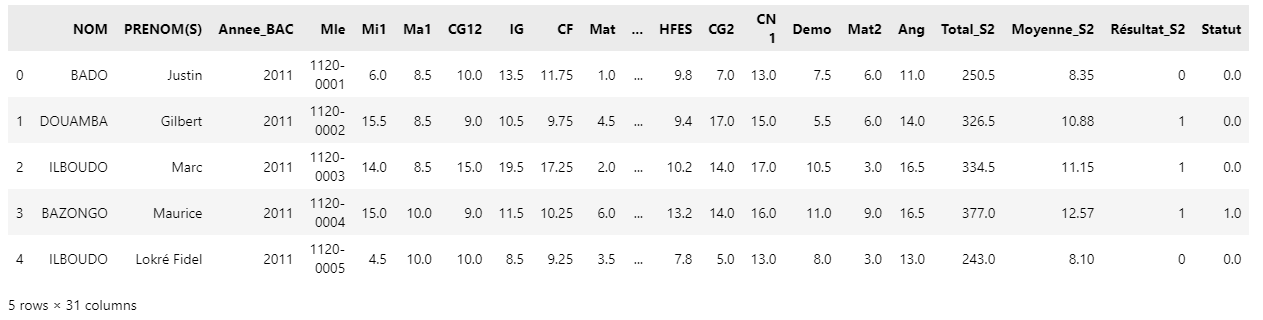
\includegraphics[width=11cm,height=3cm]{images/Dataset.png}%
    \caption{Présentation du Dataset.}%
\end{table}

Sur l’ensemble de ces données, nous avons un manque de données au niveau de la variable cible, soit environ 36\% des données sont manquantes. Ce manque est lié à l’indisponibilité des résultats de licence des bacheliers de 2017 et 2018.
Après avoir effectué une analyse approfondie de nos données, nous avons appliqué plusieurs méthodes de prétraitement des données pour garantir la qualité et la fiabilité de nos prédictions. Cela inclut le nettoyage des données pour éliminer les valeurs aberrantes et les données manquantes, la normalisation des données pour mettre toutes les caractéristiques sur la même échelle, la sélection des caractéristiques pour éliminer les variables redondantes ou peu informatives, et la conversion des données catégorielles en format numérique si nécessaire. Ensuite, les données sont divisées en ensembles d'entraînement et de test pour évaluer les performances du modèle. En appliquant ces méthodes de prétraitement, nous avons amélioré la qualité de nos données et optimisé les performances de notre modèle de prédiction.
\begin{figure}[H]
    \centering
    \setlength{\fboxsep}{5pt}
    \setlength{\fboxrule}{0.5pt}
    \begin{minipage}[t]{0.45\textwidth}
        \centering
        \fbox{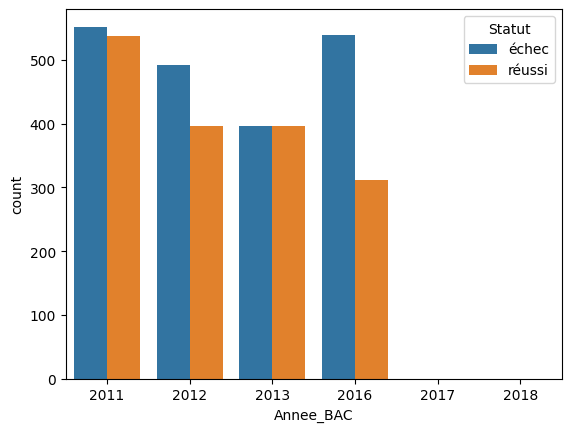
\includegraphics[width=7cm,height=5cm]{images/1.png}}
        \caption{Histogramme des valeurs manquantes pour les BAC 2017 et BAC 2018 avant le prétraitement.}
    \end{minipage}\hfill
    \begin{minipage}[t]{0.45\textwidth}
        \centering
        \fbox{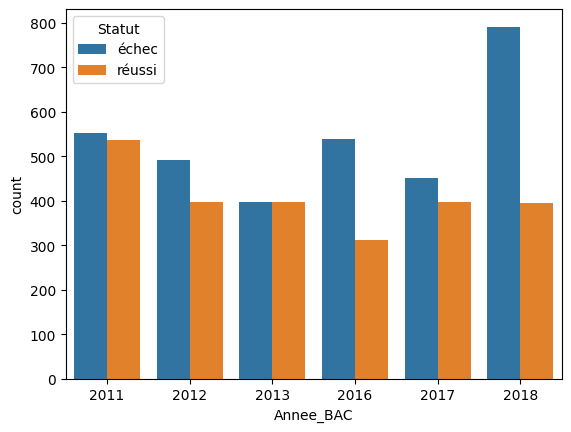
\includegraphics[width=7cm,height=5cm]{images/2.png}}
        \caption{Histogramme des valeurs manquantes pour les BAC 2017 et BAC 2018 après le prétraitement.}
    \end{minipage}
\end{figure}


\subsection{Entraînement du modèle}
L'étape d'entraînement du modèle implique de présenter les données d'entraînement à chacun des algorithmes sélectionnés et d'ajuster leurs paramètres en utilisant différentes techniques d'optimisation adaptées à chaque algorithme.
Les algorithmes entraînés sont entre autres:

\subsubsection{K plus proches voisins (KNN)}
L'algorithme des k plus proches voisins, également connu sous le nom de KNN ou k-NN, est un discriminant d'apprentissage supervisé non paramétrique, qui utilise la proximité pour effectuer des classifications ou des prédictions sur le regroupement d'un point de données individuel. Bien qu'il puisse être utilisé pour des problèmes de régression ou de classification, il est généralement utilisé comme algorithme de classification, en partant de l'hypothèse que des points similaires peuvent être trouvés les uns à côté des autres.
\begin{figure}[H]%
    \center%
    \setlength{\fboxsep}{5pt}%
    \setlength{\fboxrule}{0.5pt}%
    \fbox{
    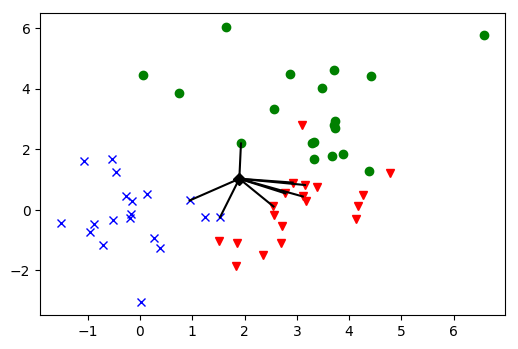
\includegraphics[width=11cm,height=6cm]{images/KNN.png}%
    }
    \caption{K plus proches voisins.}%
\end{figure}


\subsubsection{Machines à vecteurs de support (SVM)}
Les machines à vecteurs de support, de l'anglais Support Vector Machines, sont aussi appelées Séparateur à Vaste Marge. Ce sont des algorithmes d'apprentissage qui servent à prévoir une variable quantitative. Elles permettent de classer ou séparer les données en étant le plus éloigné possible des observations. En effet, il peut y avoir une infinité de séparateurs possibles. Le meilleur hyperplan est, selon les SVMs celui qui maximise les marges avec les objets de chaque catégorie.
\begin{figure}[H]%
    \center%
    \setlength{\fboxsep}{5pt}%
    \setlength{\fboxrule}{0.5pt}%
    \fbox{
    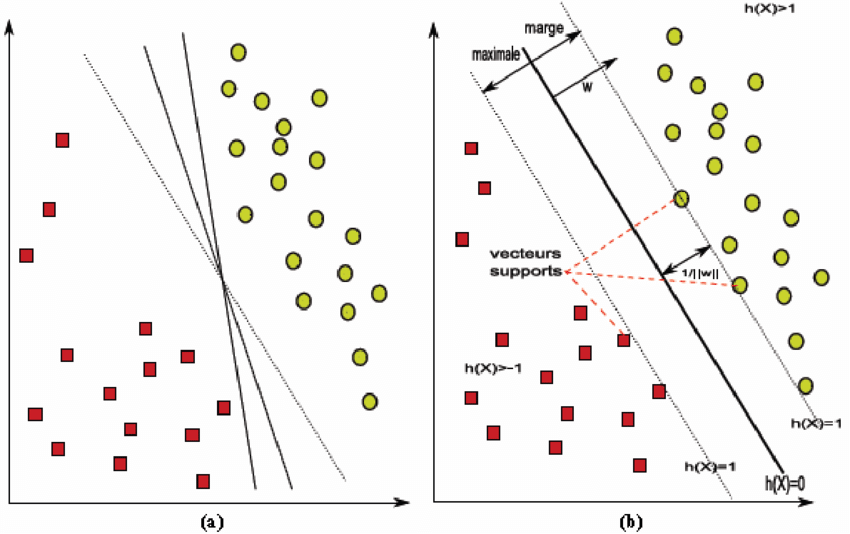
\includegraphics[width=12cm,height=7cm]{images/Principe-des-SVM.png}%
    }
    \caption{Machines à vecteurs de support.}%
\end{figure}

\subsubsection{Arbres de décision}
Les arbres de décision sont un modèle de prédiction qui peut être représenté sous la forme d’un arbre. Chaque nœud de l’arbre teste une condition sur une variable et chacun de ses enfants correspond à une réponse possible à cette condition. Les feuilles de l’arbre correspondent à une étiquette.
Pour prédire l’étiquette d’une observation, on « suit » les réponses aux tests depuis la racine de l’arbre, et on retourne l’étiquette de la feuille à laquelle on arrive.
\begin{figure}[H]%
    \center%
    \setlength{\fboxsep}{5pt}%
    \setlength{\fboxrule}{0.5pt}%
    \fbox{
    \includegraphics[width=12cm,height=5cm]{images/abre de décision.png}%
    }
    \caption{Exemple d’arbre de décision pour étiqueter un fruit.}%
\end{figure}

\subsubsection{Réseaux de neurones artificiels}
Les réseaux de neurones, également connus sous le nom de réseaux de neurones artificiels (ANN) ou réseaux de neurones simulés sont au cœur des algorithmes de l'apprentissage en profondeur. Leur nom et leur structure sont inspirés du cerveau humain, imitant la manière dont les neurones biologiques s'envoient des signaux.
Les réseaux de neurones artificiels sont constitués de couches nodales, contenant une couche d'entrée, une ou plusieurs couches cachées et une couche de sortie. Chaque nœud, ou neurone artificiel, se connecte à un autre et possède un poids et un seuil associés. Si la sortie d'un nœud est supérieure à la valeur de seuil spécifiée, ce nœud est activé et envoie des données à la couche suivante du réseau. Sinon, aucune donnée n'est transmise à la couche suivante du réseau.
\begin{figure}[H]%
    \center%
    \setlength{\fboxsep}{5pt}%
    \setlength{\fboxrule}{0.5pt}%
    \fbox{
    \includegraphics[width=10cm,height=6cm]{images/Réseaux de neurones.png}%
    }
    \caption{Réseaux de neurones artificiels.}%
\end{figure}

\subsubsection{Adaboost}
L'algorithme AdaBoost, ou Adaptive Boosting, est une technique d'apprentissage automatique utilisée principalement pour la classification. Son principe de fonctionnement repose sur l'idée de combiner plusieurs classificateurs faibles pour former un classificateur fort. Initialement, chaque exemple de formation se voit attribuer un poids égal. Ensuite, AdaBoost itère sur les données d'entraînement, en accordant une attention particulière aux exemples mal classés par les classificateurs précédents. À chaque itération, un nouveau classificateur faible est entraîné, et les poids des exemples sont mis à jour en fonction de leurs erreurs de classification. Les classificateurs faibles sont ensuite pondérés en fonction de leur performance, et leur combinaison conduit à un classificateur global.
\begin{figure}[H]%
    \center%
    \setlength{\fboxsep}{5pt}%
    \setlength{\fboxrule}{0.5pt}%
    \fbox{
    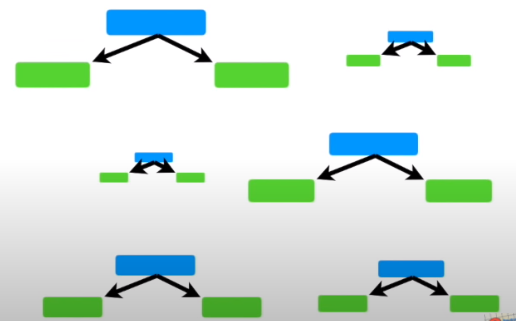
\includegraphics[width=10cm,height=6cm]{images/Adaboost img.png}%
    }
    \caption{Adaboost.}%
\end{figure}

\subsubsection{Forêt aléatoire}
La forêt aléatoire est un algorithme d'apprentissage automatique utilisé pour la classification, la régression et d'autres tâches. Elle appartient à la famille des méthodes d'ensemble, tout comme AdaBoost. La forêt aléatoire crée un ensemble de nombreux arbres de décision, où chaque arbre est formé sur un sous-ensemble aléatoire des données d'entraînement et utilise une sélection aléatoire des caractéristiques à chaque nœud de décision. L'idée principale derrière la forêt aléatoire est que la combinaison des prédictions de plusieurs arbres de décision réduit le surapprentissage et améliore la performance prédictive du modèle global.
\begin{figure}[H]%
    \center%
    \setlength{\fboxsep}{5pt}%
    \setlength{\fboxrule}{0.5pt}%
    \fbox{
    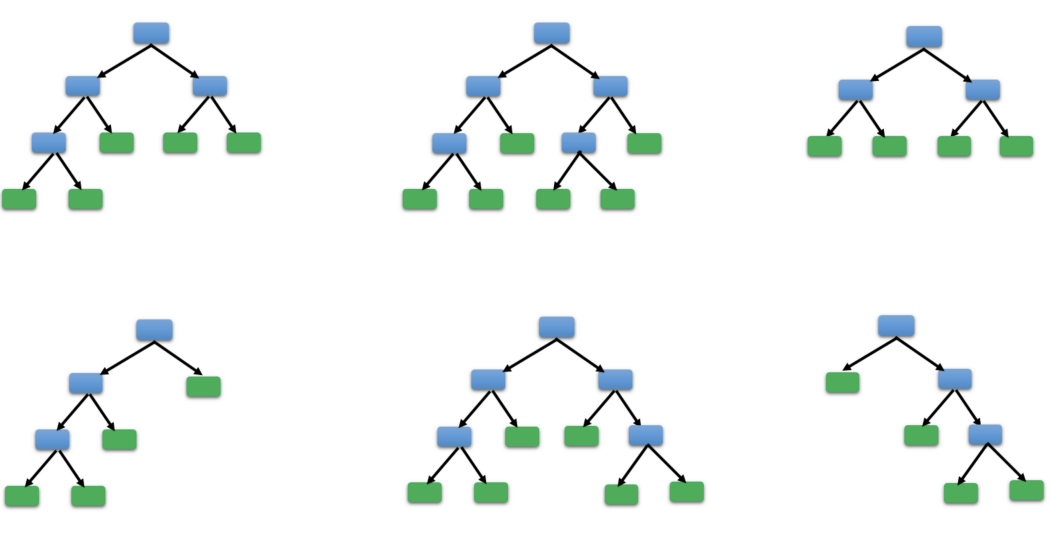
\includegraphics[width=10cm,height=6cm]{images/rand_forest_illustration.png}%
    }
    \caption{Forêt aléatoire.}%
\end{figure}

Chaque algorithme apprend à partir des exemples d'entraînement en ajustant ses paramètres internes de manière à minimiser la fonction de perte spécifique à chaque algorithme, ce qui lui permet de généraliser et de faire des prédictions précises sur de nouvelles données.

\section{Conclusion}
Ce chapitre nous a permis d'explorer l'état de l'art sur la prédiction de la réussite des étudiants, en examinant les études antérieures, les méthodes et techniques utilisées, ainsi que les limitations des approches existantes. Nous avons également présenté une approche de solution visant à prédire le succès universitaire des étudiants orientés en économie, en utilisant l'intelligence artificielle, et la modélisation de cette solution, notamment le choix du modèle, la méthode de prétraitement des données et l'entraînement du modèle, offrant ainsi un aperçu de la méthodologie à suivre pour mener à bien cette prédiction.

    
    \chapter{IMPLÉMENTATION, RÉSULTATS ET DISCUSSION}
\begin{spacing}{1.2}
\minitoc
\thispagestyle{MyStyle}
\end{spacing}
\newpage

Dans ce chapitre, nous plongeons dans l'aspect pratique de notre projet, passant de la théorie à la mise en œuvre concrète. Nous commencerons par présenter l'environnement de développement utilisé, en mettant en lumière les outils, les bibliothèques et les configurations nécessaires à l'implémentation de notre modèle de prédiction. Ensuite, nous détaillerons l'architecture de l'application de prédiction, suivie du développement de l'application Web pour une utilisation conviviale. Enfin, nous examinerons les résultats obtenus et engagerons une discussion sur ces résultats, explorant également les perspectives futures de notre projet.

\section{Environnement de développement}

\subsection{Outils de développement}
Pour la réalisation de notre projet, nous avons opté pour un ensemble d'outils de développement qui ont été sélectionnés avec soin pour leur efficacité, leur polyvalence et leur adaptabilité aux exigences de notre tâche. Nous avons principalement utilisé le langage Python, l'environnement de développement VS Code, et Jupyter Notebook. Chacun de ces outils a été choisi pour des raisons spécifiques qui seront détaillées ci-dessous :

\subsubsection{Le langage python}
Python a été choisi comme langage de programmation principal pour plusieurs raisons. Tout d'abord, c'est un langage interprété, qui n'a pas besoin d'être compilé pour être exécuté, contrairement à des langages comme le C ou le C++, et de haut niveau. Il demande relativement peu de connaissances sur le fonctionnement d'un ordinateur pour être utilisé. Ensuite, Python est multiplateforme, c'est-à-dire qu'il fonctionne sur de nombreux systèmes d'exploitation : Windows, Mac OS X, Linux, Android, iOS, depuis les mini-ordinateurs Raspberry Pi jusqu'aux supercalculateurs. De plus, Python bénéficie d'une vaste bibliothèque de modules spécialisés pour le machine learning et le traitement de données par rapport à d'autres langages (Java, C++), tels que TensorFlow, Scikit-learn, PyTorch et Pandas, ce qui facilite grandement le développement de modèles d'intelligence artificielle. En outre, la communauté Python active et engagée offre un support continu ainsi qu'un accès à une multitude de ressources et de tutoriels, ce qui a été un atout précieux tout au long de notre projet.

\subsubsection{Visual Studio Code (VS Code)}
VS Code s'est imposé comme un environnement de développement de premier choix en raison de sa légèreté, de sa rapidité et de sa richesse en fonctionnalités. Son interface utilisateur intuitive et personnalisable offre une expérience de développement fluide, tout en offrant un large éventail d'extensions pour répondre à divers besoins de développement. De plus, VS Code prend en charge plusieurs langages de programmation, ce qui en fait un choix polyvalent pour travailler sur des projets multidisciplinaires. Enfin, la prise en charge native de Git et d'autres outils de contrôle de version a facilité la collaboration et la gestion du code source tout au long du cycle de développement.

\subsubsection{Jupyter Notebook}
Jupyter Notebook est une application Web open source qui permet de créer et de partager des documents comprenant du code en direct, des équations et d'autres ressources multimédias, utilisés dans plus de 40 langages de programmation, dont Python, Julia, Ruby, R, ou encore Scala. Nous l'avons utilisé dans notre projet pour l'analyse exploratoire des données ainsi que la modélisation statistique. Facile à utiliser, il permet d'exécuter le code cellule par cellule pour mieux comprendre son fonctionnement.

\subsection{Bibliothèques et librairie utilisées}
Dans le cadre de notre projet visant à prédire la réussite en licence des étudiants orientés en SEG à l'aide de l'intelligence artificielle, nous avons utilisé plusieurs bibliothèques Python spécialisées. Ces bibliothèques sont des outils essentiels pour la manipulation, l'analyse, la visualisation des données et la mise en œuvre des modèles d'apprentissage automatique. 

\subsubsection{NumPy}
NumPy est une bibliothèque fondamentale pour le calcul numérique en Python. Elle fournit des structures de données de tableau multidimensionnel (arrays) efficaces et performantes, ainsi que des fonctions mathématiques pour effectuer des opérations sur ces tableaux. Dans notre projet, NumPy est utilisé en combinaison avec Pandas pour effectuer des opérations de manipulation et de transformation de données plus rapides et efficaces. Les tableaux NumPy sont utilisés pour stocker et traiter les données avant de les convertir en DataFrames Pandas. De plus, NumPy est souvent utilisé en conjonction avec d'autres bibliothèques telles que Matplotlib et Scikit-learn pour effectuer des opérations mathématiques et des calculs numériques nécessaires à l'analyse des données et à la modélisation. En résumé, NumPy est une bibliothèque essentielle qui améliore les performances et la productivité lors de la manipulation et de l'analyse des données dans notre projet.

\subsubsection{Pandas}
Pandas est une bibliothèque open-source largement utilisée pour la manipulation et l'analyse des données en Python. Son principal objet est le DataFrame, une structure de données tabulaire puissante et flexible. Dans notre projet, Pandas est essentiel pour charger, nettoyer et prétraiter les données. Nous utilisons Pandas pour importer les jeux de données, traiter les valeurs manquantes, supprimer les doublons, filtrer les données et réaliser des opérations de fusion et de regroupement. Grâce à ses fonctionnalités avancées, Pandas simplifie la manipulation des données, ce qui permet un workflow plus fluide lors de la préparation des données pour l'analyse et la modélisation.

\subsubsection{Matplotlib}
Matplotlib est une bibliothèque de visualisation de données en Python qui permet de créer une grande variété de graphiques statiques, notamment des graphiques linéaires, des diagrammes à barres, des diagrammes circulaires, des histogrammes, etc. Dans notre projet, Matplotlib est utilisé pour visualiser les données d'entraînement et de test, ainsi que les résultats de la modélisation. Nous pouvons créer des graphiques pour explorer la distribution des variables, analyser les relations entre les caractéristiques et la variable cible, et évaluer les performances du modèle. Matplotlib offre une flexibilité et une personnalisation étendue, ce qui nous permet de créer des visualisations informatives et esthétiques pour communiquer nos résultats de manière efficace.

\subsubsection{Seaborn}
Seaborn est une bibliothèque de visualisation de données basée sur Matplotlib qui offre une interface plus conviviale et des styles de tracé esthétiques par défaut. Elle permet de créer rapidement des graphiques complexes et informatifs, notamment des diagrammes en violon, des tracés de régression linéaire et des matrices de corrélation. Dans notre projet, Seaborn complète Matplotlib en offrant des fonctionnalités supplémentaires pour explorer et visualiser les relations entre les variables. Nous utilisons Seaborn pour créer des graphiques qui mettent en évidence les tendances, les modèles et les corrélations dans nos données, ce qui nous aide à mieux comprendre le comportement des variables et à prendre des décisions plus éclairées lors de la modélisation.

\subsubsection{Scikit-learn}
Scikit-learn est une bibliothèque d'apprentissage automatique open-source qui offre une large gamme d'algorithmes d'apprentissage supervisé et non supervisé, ainsi que des outils pour l'évaluation et la validation des modèles. Dans notre projet, nous utilisons Scikit-learn pour construire, entraîner et évaluer notre modèle de prédiction. Nous avons choisi Scikit-learn pour sa simplicité d'utilisation, sa cohérence d'interface et sa grande efficacité. De plus, Scikit-learn propose une documentation exhaustive et une communauté active, ce qui en fait un choix populaire pour le développement d'applications d'apprentissage automatique en Python.

\subsubsection{Flask}
Flask est un framework web minimaliste pour Python qui permet de créer des applications Web légères et flexibles. Dans notre projet, nous utilisons Flask pour développer une interface utilisateur Web qui permettra aux utilisateurs de saisir les données et de générer des prédictions à partir du modèle entraîné. Flask offre des fonctionnalités pour gérer les requêtes HTTP, générer des pages Web dynamiques et interagir avec les modèles Python en arrière-plan. Nous avons choisi Flask pour sa simplicité, sa flexibilité et sa compatibilité avec les autres outils utilisés dans notre projet.

\subsection{Configuration des Outils et des Paramètres}
Pour garantir un développement efficace, nous avons configuré nos outils et nos paramètres selon les besoins spécifiques de notre projet. Cela comprend la configuration des environnements virtuels Python pour gérer les dépendances du projet, l'installation des extensions appropriées dans VS Code pour améliorer la productivité des développeurs, l'optimisation des paramètres de Jupyter Notebook pour assurer des performances optimales lors de l'exécution de code par cellules, et la configuration de Git comme système de contrôle de version pour notre projet qui nous a permis de gérer les différentes versions de notre code source et de suivre les modifications apportées aux fichiers.

\section{Présentation du modèle implémenté}
Après avoir développé une approche de solution dans le chapitre précédent, nous entrons maintenant dans la phase de concrétisation avec la présentation du modèle implémenté. Cette section se concentre sur la description détaillée de l'architecture de l'application de prédiction, la construction et les caractéristiques du modèle, ainsi que le développement de l'application web associée.

\subsection{Architecture du modèle implémenté}
L'architecture de notre modèle implémenté repose sur une approche modulaire et évolutive, conçue pour gérer efficacement les différentes étapes du processus de prédiction. Notre application est divisée en trois modules principaux : le module de prétraitement des données, le module de construction et d'entraînement du modèle, et le module de déploiement de l'application Web. 
\begin{itemize} 
	\item[\ding{118}] \textbf{Module de prétraitement des données} : il est chargé de nettoyer, normaliser et préparer les données brutes avant de les utiliser pour l'entraînement du modèle. Il comprend des fonctions pour détecter et traiter les valeurs aberrantes, gérer les données manquantes. 
	\item[\ding{118}] \textbf{Module de construction et d'entraînement du modèle} : ce module est responsable de la construction du modèle de prédiction à partir des données prétraitées. Il utilise des algorithmes d'apprentissage automatique cité dans le chapitre précédent. 
	\item[\ding{118}] \textbf{Module de déploiement de l'application web} : ce module prend en charge le déploiement de l'application web permettant aux utilisateurs de soumettre de nouvelles données et d'obtenir des prédictions en temps réel. 
\end{itemize}

\subsection{Implémentation du modèle}
 La mise en œuvre du modèle de prédiction repose sur les choix effectués lors de la phase de modélisation précédente. Nous utilisons les bibliothèques et les outils de développement mentionnés dans la section précédente pour entraîner le modèle sur les données prétraitées. Cette étape comprend la création d'un pipeline de prétraitement des données pour assurer la cohérence et la qualité des entrées du modèle. Nous explorons également les paramètres du modèle et les techniques d'optimisation pour améliorer ses performances prédictives.

\subsection{Développement de l’application Web} Le développement de notre application Web s'est appuyé sur le framework Flask pour sa simplicité, sa flexibilité et sa puissance. Nous avons utilisé Flask pour créer une API RESTful qui gère les requêtes des utilisateurs et communique avec notre modèle de prédiction. En plus de Flask, nous avons également utilisé HTML, CSS et Bootstrap pour concevoir et styliser l'interface utilisateur de l'application Web. Ainsi, l'application Web permet aux utilisateurs de soumettre des données sur les étudiants et d'obtenir des prédictions sur leur statut de réussite en temps réel. L'interface utilisateur est conviviale et intuitive, offrant une expérience utilisateur fluide et agréable.

\section{Résultats et discussions}

\subsection{Métrique et évaluation des modèles entraînés}
Pour évaluer l'efficacité de notre modèle de prédiction, nous avons utilisé plusieurs métriques de performance couramment utilisées dans le domaine de l'apprentissage automatique. Parmi ces métriques, nous avons notamment examiné la précision, le rappel, la F1-score et la matrice de confusion. Ces mesures nous ont permis d'évaluer la capacité du modèle à prédire avec précision la réussite en licence des étudiants orientés en économie. Les résultats obtenus sont présentés en détail dans les lignes qui suivent.

\subsubsection{Métrique de la performance}
\subsubsection*{Précision} La précision est une mesure qui évalue la proportion d'observations positives correctement prédites par le modèle parmi toutes les observations prédites comme positives. En d'autres termes, elle indique la capacité du modèle à éviter les faux positifs. Dans notre projet, la précision est cruciale, car elle nous permet de déterminer avec quelle fiabilité le modèle identifie correctement les étudiants qui réussissent effectivement leur licence. La formule de la précision est définie comme suit : \[ \text{Précision} = \frac{\text{Vrai\ Positif}}{\text{Vrai\ Positif} + \text{Faux\ Positif}} \]

\subsubsection*{Rappel} Le rappel, également appelé sensibilité ou recall en anglais, mesure la proportion d'observations positives correctement identifiées par le modèle parmi toutes les observations positives réelles. Il est important dans notre projet, car il nous indique la capacité du modèle à détecter les véritables positifs, c'est-à-dire les étudiants qui réussissent effectivement leur licence. La formule du rappel est la suivante : \[ \text{Rappel} = \frac{\text{Vrai\ Positif}}{\text{Vrai\ Positif} + \text{Faux\ Négatif}} \]

\subsubsection*{F1-Score}
Le F1-Score est une mesure qui combine à la fois la précision et le rappel en une seule valeur, offrant ainsi un équilibre entre les deux. Il est particulièrement utile lorsque les classes sont déséquilibrées, comme c'est souvent le cas dans les problèmes de classification binaire. Dans notre projet, le F1-Score nous permet d'évaluer globalement la performance du modèle en termes de précision et de rappel. La formule du F1-Score est définie comme suit :
\[ F1 = 2 \times \frac{\text{Précision} \times \text{Rappel}}{\text{Précision} + \text{Rappel}} \]

\subsubsection*{Matrice de confusion}
La matrice de confusion est une représentation tabulaire des prédictions du modèle par rapport aux valeurs réelles de la variable cible. Elle permet de visualiser les performances du modèle en termes de vrais positifs, vrais négatifs, faux positifs et faux négatifs. Cette métrique est essentielle dans notre projet, car elle fournit une vue détaillée des performances du modèle pour chaque classe de prédiction. La matrice de confusion n'a pas de formule spécifique, mais elle est générée à partir des prédictions du modèle et des valeurs réelles.

La matrice de confusion est une métrique essentielle qui permet d'évaluer les performances d'un modèle de prédiction en termes de vrais positifs, faux positifs, vrais négatifs et faux négatifs. Ces différentes classifications sont définies comme suit :

\begin{itemize}
	 \item[\ding{118}] \textbf{Vrai Positif (VP)} : cela correspond aux cas où le modèle prédit correctement qu'un étudiant a réussi sa licence et que cet étudiant a effectivement réussi.
	\item[\ding{118}] \textbf{Faux Positif (FP)} : dans ce cas, le modèle prédit à tort qu'un étudiant a réussi sa licence, alors qu'en réalité, cet étudiant a échoué.
	\item[\ding{118}] \textbf{Vrai Négatif (VN)} : ce sont les cas où le modèle prédit correctement qu'un 	étudiant a échoué à sa licence et que cet étudiant a effectivement échoué.
	\item[\ding{118}] \textbf{Faux Négatif (FN)} : Il s'agit des cas où le modèle prédit à tort qu'un étudiant a échoué à sa licence alors qu'en réalité, cet a effectivement réussi.
\end{itemize}

\begin{table}[H]%
    \center%
    \setlength{\fboxsep}{5pt}%
    \setlength{\fboxrule}{0.5pt}%
    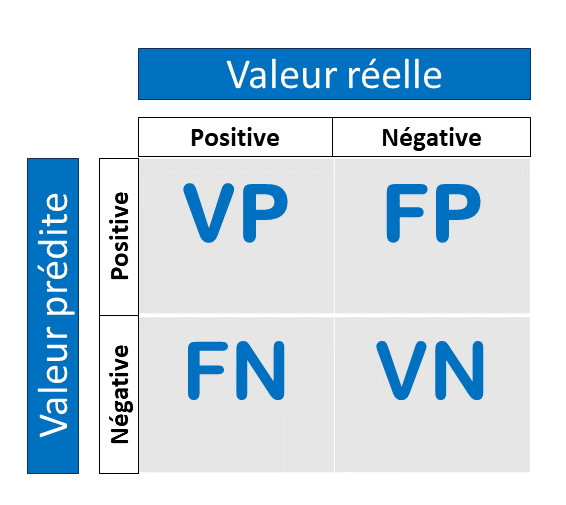
\includegraphics[width=9cm,height=6cm]{images/matrice de confusion.png}%
    \caption{Matrice de confusion.}%
\end{table}

\subsubsection{Évaluation des algorithmes entraînés}
Nous avons évalué les performances de nos différents algorithmes à l'aide des métriques d'évaluation précédemment définies afin de sélectionner celui offrant les meilleures prédictions. Cette évaluation s'est accompagnée de la génération de courbes et de graphiques pour une visualisation complète et comparative des performances des algorithmes.

\subsubsection*{Random Forest ou Forêt aléatoire}
\begin{minipage}[t]{0.5\textwidth}
    \begin{table}[H]
        \centering
        \setlength{\fboxsep}{5pt}
        \setlength{\fboxrule}{0.5pt}
        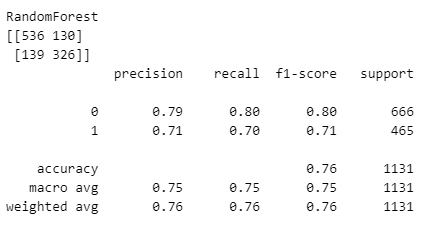
\includegraphics[width=7cm,height=5.4cm]{images/RandomForest.png}
        \caption{Matrice de confusion de Random Forest.}
    \end{table}
\end{minipage}
\begin{minipage}[t]{0.5\textwidth}
    \begin{figure}[H]
        \centering
        \setlength{\fboxsep}{5pt}
        \setlength{\fboxrule}{0.5pt}
        \fbox{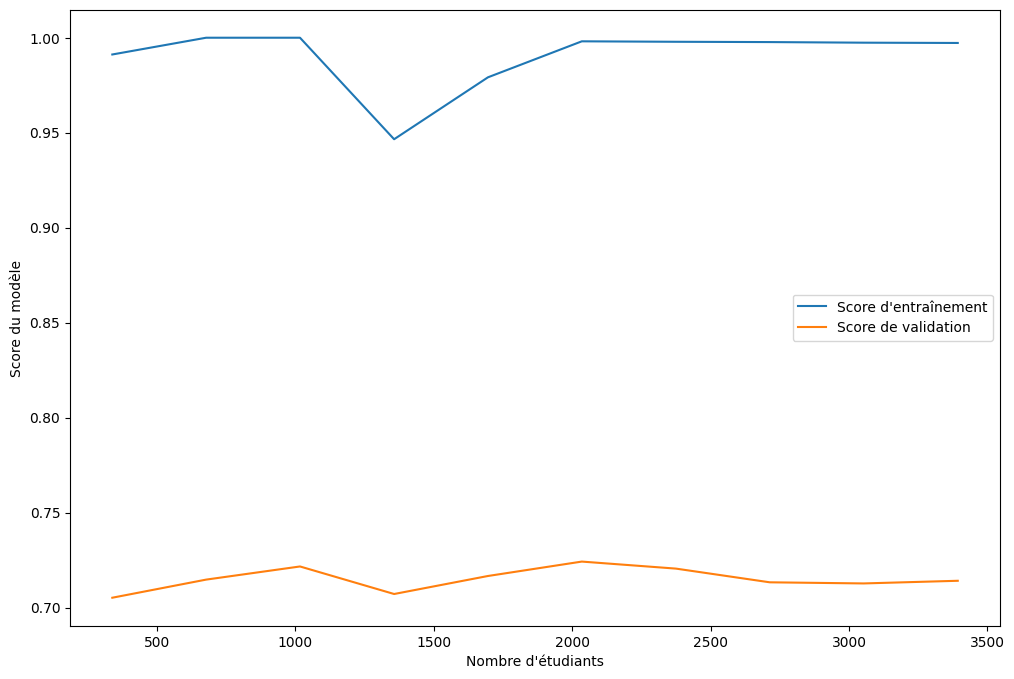
\includegraphics[width=7cm,height=5cm]{images/Evaluation RandomForest.png}}
        \caption{Courbe d'évaluation de Random Forest.}
    \end{figure}
\end{minipage}

\subsubsection*{Adaboost}
\begin{minipage}[t]{0.5\textwidth}
    \begin{table}[H]
        \centering
        \setlength{\fboxsep}{5pt}
        \setlength{\fboxrule}{0.5pt}
        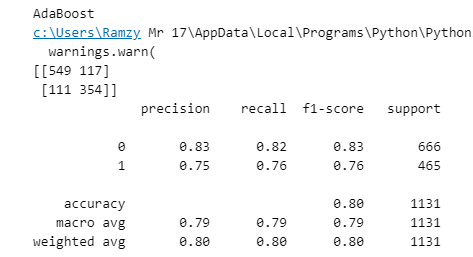
\includegraphics[width=7cm,height=5.36cm]{images/Adaboost.png}
        \caption{Matrice de confusion de Adaboost.}
    \end{table}
\end{minipage}
\begin{minipage}[t]{0.5\textwidth}
    \begin{figure}[H]
        \centering
        \setlength{\fboxsep}{5pt}
        \setlength{\fboxrule}{0.5pt}
        \fbox{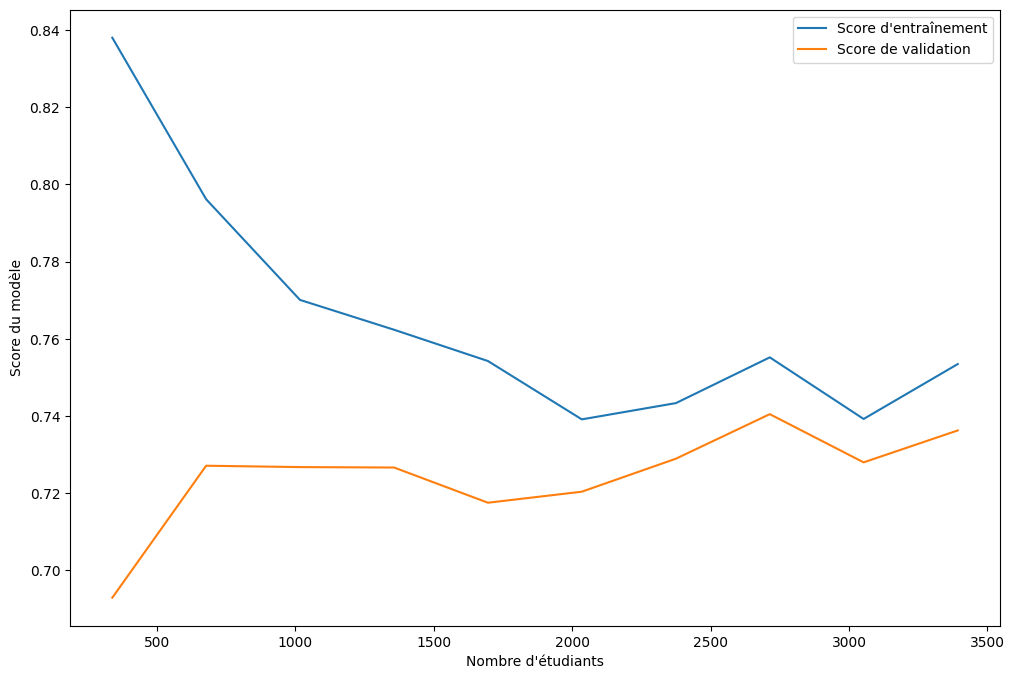
\includegraphics[width=7cm,height=5cm]{images/Evaluation Adaboost.png}}
        \caption{Courbe d'évaluation de Adaboost.}
    \end{figure}
\end{minipage}

\subsubsection*{SVM}
\begin{minipage}[t]{0.5\textwidth}
    \begin{table}[H]
        \centering
        \setlength{\fboxsep}{5pt}
        \setlength{\fboxrule}{0.5pt}
        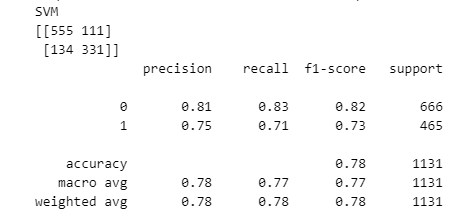
\includegraphics[width=7cm,height=5.36cm]{images/SVM.png}
        \caption{Matrice de confusion de SVM.}
    \end{table}
\end{minipage}
\begin{minipage}[t]{0.5\textwidth}
    \begin{figure}[H]
        \centering
        \setlength{\fboxsep}{5pt}
        \setlength{\fboxrule}{0.5pt}
        \fbox{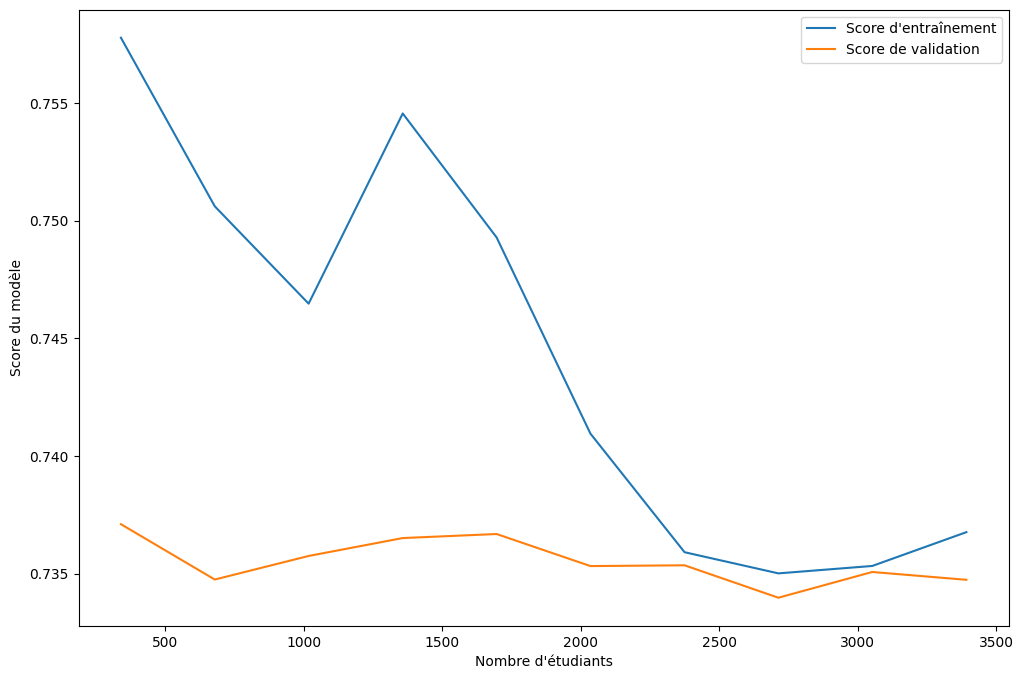
\includegraphics[width=7cm,height=5cm]{images/Evaluation SVM.png}}
        \caption{Courbe d'évaluation de SVM.}
    \end{figure}
\end{minipage}

\subsubsection*{KNN}
\begin{minipage}[t]{0.5\textwidth}
    \begin{table}[H]
        \centering
        \setlength{\fboxsep}{5pt}
        \setlength{\fboxrule}{0.5pt}
        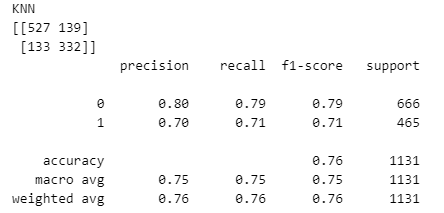
\includegraphics[width=7cm,height=5.37cm]{images/KNN (1).png}
        \caption{Matrice de confusion de KNN.}
    \end{table}
\end{minipage}
\begin{minipage}[t]{0.5\textwidth}
    \begin{figure}[H]
        \centering
        \setlength{\fboxsep}{5pt}
        \setlength{\fboxrule}{0.5pt}
        \fbox{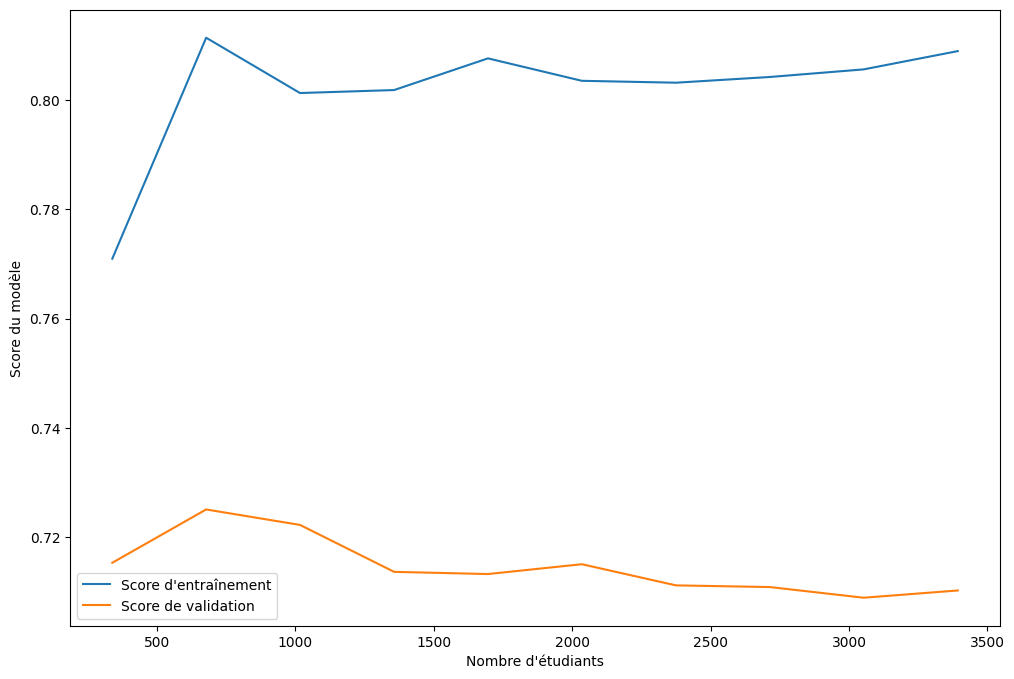
\includegraphics[width=7cm,height=5cm]{images/Evaluation KNN.png}}
        \caption{Courbe d'évaluation de KNN.}
    \end{figure}
\end{minipage}
\newpage
\subsubsection*{Arbre de décision}
\begin{minipage}[t]{0.5\textwidth}
    \begin{table}[H]
        \centering
        \setlength{\fboxsep}{5pt}
        \setlength{\fboxrule}{0.5pt}
        \includegraphics[width=7cm,height=5.37cm]{images/Abre de décision.png}
        \caption{Matrice de confusion de Arbre de décision.}
    \end{table}
\end{minipage}
\begin{minipage}[t]{0.5\textwidth}
    \begin{figure}[H]
        \centering
        \setlength{\fboxsep}{5pt}
        \setlength{\fboxrule}{0.5pt}
        \fbox{\includegraphics[width=7cm,height=5cm]{images/Evaluation Abre de décision.png}}
        \caption{Courbe d'évaluation de Arbre de décision.}
    \end{figure}
\end{minipage}

\subsubsection*{Réseaux de neurones}
\begin{minipage}[t]{0.5\textwidth}
    \begin{table}[H]
        \centering
        \setlength{\fboxsep}{5pt}
        \setlength{\fboxrule}{0.5pt}
        \includegraphics[width=7cm,height=5.37cm]{images/Réseau de neurones.png}
        \caption{Matrice de confusion de Réseaux de neurones.}
    \end{table}
\end{minipage}
\begin{minipage}[t]{0.5\textwidth}
    \begin{figure}[H]
        \centering
        \setlength{\fboxsep}{5pt}
        \setlength{\fboxrule}{0.5pt}
        \fbox{\includegraphics[width=7cm,height=5cm]{images/Evaluation Réseau de neurones.png}}
        \caption{Courbe d'évaluation de Réseaux de neurones.}
    \end{figure}
\end{minipage}
\newpage
Nous pouvons résumer les métriques d'évaluation des différents algorithmes dans le tableau ci-dessous :

\begin{table}[h]
\centering
\begin{tabular}{lccc}
\hline
Algorithme & Précision & Rappel & F1-score \\
\hline
\textit{Random Forest} & 75\% & 75\% & 75\% \\
\textit{Adaboost} & 79\% & 79\% & 79\% \\
\textit{SVM} & 78\% & 77\% & 77\% \\
\textit{KNN} & 75\% & 75\% & 75\% \\
\textit{Arbre de décision} & 71\% & 71\% & 71\% \\
\textit{Réseaux de neurones} & 80\% & 80\% & 80\% \\
\hline
\end{tabular}
\caption{Métriques d'évaluation des algorithmes.}

\end{table}

L'analyse du tableau des métriques d'évaluation des différents algorithmes permet de comparer les performances de chaque algorithme en termes de précision, rappel et F1-score. Ces observations suggèrent que les réseaux de neurones pourraient être l'algorithme le plus prometteur pour la tâche spécifique évaluée, en raison de leur performance globalement supérieure sur les trois métriques d'évaluation. Il est important de noter que ces résultats serviront de base pour l'optimisation future des hyperparamètres, permettant ainsi d'améliorer davantage les performances des algorithmes et ce que nous obtenons.

\begin{minipage}[t]{0.5\textwidth}
    \begin{table}[H]
        \centering
        \setlength{\fboxsep}{5pt}
        \setlength{\fboxrule}{0.5pt}
        \includegraphics[width=7cm,height=5.37cm]{images/Réseau de neurone opti.png}
        \caption{Matrice de confusion de Réseaux de neurones avec les hyperparamètres.}
    \end{table}
\end{minipage}
\begin{minipage}[t]{0.5\textwidth}
    \begin{figure}[H]
        \centering
        \setlength{\fboxsep}{5pt}
        \setlength{\fboxrule}{0.5pt}
        \fbox{\includegraphics[width=7cm,height=5cm]{images/Validation Réseau de neurone.png}}
        \caption{Courbe d'évaluation de Réseaux de neurones.}
    \end{figure}
\end{minipage}

\subsection{Déploiement du modèle}
Après avoir opté pour le modèle des Réseaux de neurones, nous l'avons déployé en utilisant la technologie Web. L'objectif de cette démarche était de développer une interface graphique permettant de visualiser les résultats des tests du modèle retenu. Cela visait à offrir aux nouveaux étudiants de l'UNZ, souhaitant évaluer leurs chances de réussite en licence économie, la possibilité de prédire leur succès. Ainsi, nous avons élaboré une interface Web basée sur Flask. La capture d'écran ci-dessous présente la page d'accueil, permettant aux utilisateurs d'exploiter le modèle pour prédire leurs chances de réussite.

\begin{figure}[H]%
    \center%
    \setlength{\fboxsep}{5pt}%
    \setlength{\fboxrule}{0.5pt}%
    \fbox{
    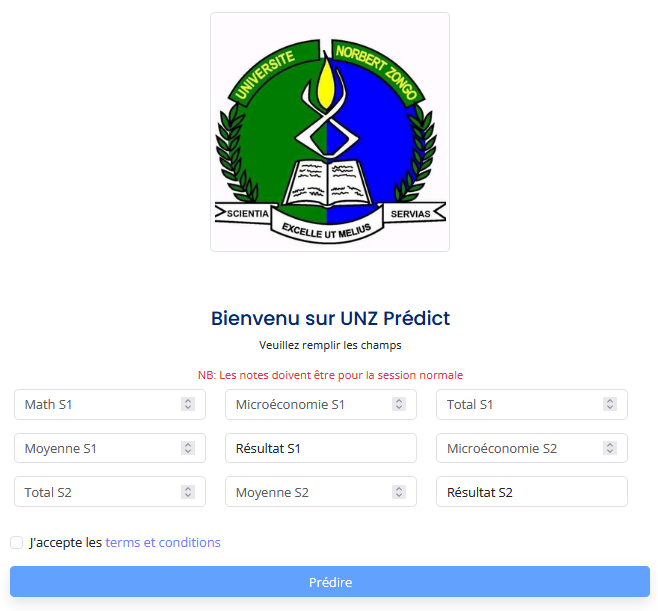
\includegraphics[width=10cm,height=11cm]{images/Unz predict.png}%
    }
    \caption{Page d’accueil de l’application Web.}%
\end{figure}
Une fois sur la page d'accueil présentée ci-dessus, l'utilisateur remplira le formulaire puis cliquera sur le bouton "Prédire". Il est à noter que les champs de ce formulaire sont des zones de saisie ou "input".

\subsection{Résultat de l'application}
Avant de mettre en production une application destinée à aider les étudiants à évaluer leurs chances de réussite en licence économie à l'UNZ, il est essentiel de la soumettre à des tests rigoureux pour garantir son bon fonctionnement et sa fiabilité. Dans cette section, nous décrirons en détail les différents tests auxquels l'application a été soumise, ainsi que les résultats obtenus. Ces tests ont été réalisés dans le but d'assurer que l'application réponde aux attentes des utilisateurs et fournisse des prédictions précises et pertinentes pour leur réussite académique.

\begin{figure}[H]%
    \center%
    \setlength{\fboxsep}{5pt}%
    \setlength{\fboxrule}{0.5pt}%
    \fbox{
    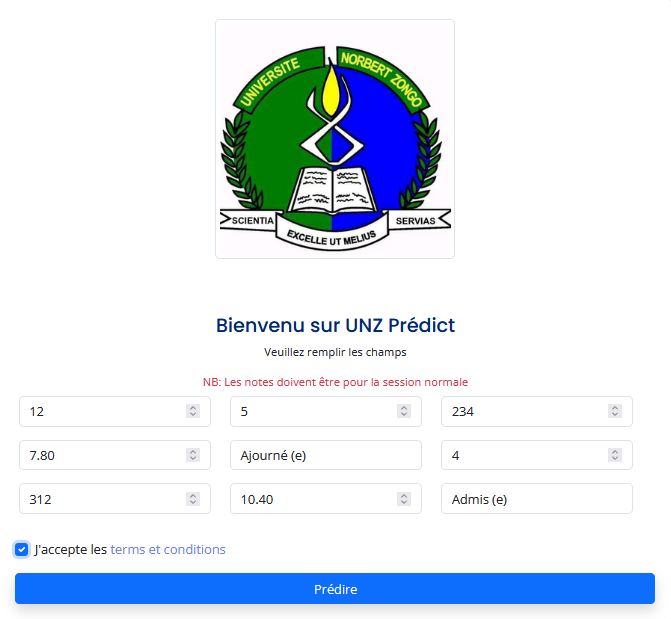
\includegraphics[width=8cm,height=9cm]{images/Forme1.png}%
    }
    \caption{Exemple de prédiction 1.}%
\end{figure}

\begin{figure}[H]%
    \center%
    \setlength{\fboxsep}{5pt}%
    \setlength{\fboxrule}{0.5pt}%
    \fbox{
    \includegraphics[width=8cm,height=9cm]{images/Résultat1.png}%
    }
    \caption{Résultat de la prédiction 1.}%
\end{figure}

Pour le cas de l'exemple de la figure 4.9, il s'agit d'un étudiant dont les résultats sont les suivants : 12 en mathématiques au semestre 1, 5 en microéconomie au semestre 1, avec un total de 234 points et une moyenne de 7,80 au semestre 1, résultant en un échec au semestre 1. Au semestre 2, l'étudiant obtient 4 en Microéconomie, un total de 312 points et une moyenne de 10,40, ce qui conduit à une réussite au semestre 2. Le modèle de prédiction estime que cet étudiant a 20,76\% de chance de réussir sa licence, ce qui veut dire qu'il va échouer.
\begin{figure}[H]%
    \center%
    \setlength{\fboxsep}{5pt}%
    \setlength{\fboxrule}{0.5pt}%
    \fbox{
    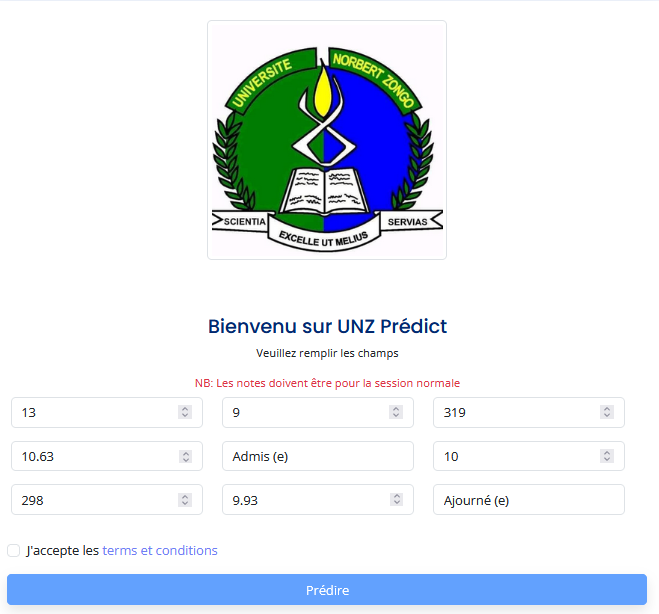
\includegraphics[width=8cm,height=9cm]{images/Forme2.png}%
    }
    \caption{Exemple de prédiction 2.}%
\end{figure}

\begin{figure}[H]%
    \center%
    \setlength{\fboxsep}{5pt}%
    \setlength{\fboxrule}{0.5pt}%
    \fbox{
    \includegraphics[width=8cm,height=9cm]{images/Résultat2.png}%
    }
    \caption{Résultat de la prédiction 2.}%
\end{figure}

Pour le cas de l'exemple de la figure 4.11, il s'agit d'un étudiant dont les résultats sont les suivants : 13 en mathématiques au semestre 1, 9 en microéconomie au semestre 1, avec un total de 319 points et une moyenne de 10.63 au semestre 1, résultant en une réussite au semestre 1. Au semestre 2, l'étudiant obtient 10 en microéconomie, un total de 298 points et une moyenne de 9.93, ce qui conduit à un échec au semestre 2. Le modèle de prédiction estime que cet étudiant a 69.14\% de chance de réussir sa licence, ce qui veut dire qu'il va réussir.

\subsection{Perspectives futures}
Enfin, en ce qui concerne les perspectives futures, nous envisageons plusieurs axes d'amélioration et d'extension de notre travail. Cela comprend l'exploration de techniques d'apprentissage automatique plus avancées, telles que les réseaux de neurones profonds, pour améliorer les performances prédictives du modèle. Nous prévoyons également d'enrichir les fonctionnalités de l'application Web en intégrant des analyses visuelles interactives et en développant des fonctionnalités de recommandation personnalisée. De plus, nous envisageons d'étendre notre étude à d'autres filières universitaires afin de généraliser notre approche à un plus large éventail de domaines.

\section{Conclusion}

Ce chapitre marque la concrétisation de notre projet, en passant de la conceptualisation à la mise en œuvre. Nous avons détaillé l'environnement de développement utilisé, l'architecture de notre application de prédiction, et présenté les résultats obtenus. En analysant ces résultats, nous avons également ouvert la porte à des perspectives futures, soulignant les opportunités d'amélioration et d'extension de notre travail. En somme, ce chapitre apporte une contribution tangible à notre projet, en le rendant opérationnel et en ouvrant la voie à de nouvelles avenues de recherche et de développement.

    
    \chapter*{CONCLUSION GÉNÉRALE}
\markboth{\MakeUppercase{CONCLUSION GÉNÉRALE}}{}
\addcontentsline{toc}{chapter}{CONCLUSION GÉNÉRALE}
\adjustmtc
\thispagestyle{MyStyle}

Le présent projet de recherche s'est attaché à explorer l'utilisation de l'intelligence artificielle comme outil de prédiction de la réussite des étudiants en licence, avec un accent particulier sur le domaine des Sciences Économiques et de Gestion à l'Université Norbert Zongo. À travers notre étude, nous avons cherché à répondre à un besoin pressant au sein de l'enseignement supérieure au Burkina Faso : celui d'identifier les étudiants en difficulté dès leur entrée à l'université et de leur fournir un soutien approprié pour maximiser leurs chances de réussite.
En analysant en profondeur l'efficacité de l'intelligence artificielle dans la prédiction de la réussite académique des étudiants en économie, nous mettons en lumière l'importance de cette approche innovante pour soutenir leur parcours académique. Notre recherche offre des perspectives précieuses pour les décideurs politiques, les administrateurs universitaires et les praticiens de l'enseignement supérieur, en identifiant les facteurs prédictifs de la réussite académique et en proposant des pistes d'action pour améliorer les résultats des étudiants.
        
    \addcontentsline{toc}{chapter}{BIBLIOGRAPHIE}
\adjustmtc
\renewcommand\bibname{BIBLIOGRAPHIE}
\begin{thebibliography}{9}
\thispagestyle{MyStyle}

\bibitem{unesco}
\textbf{Jonathan Jourde}. \emph{L'Ecole burkinabè, un condensé des défis de l'éducation en Afrique}. 2 p. 2018. UNESCO IIEP Dakar. Bureau pour l’Afrique.

\bibitem{lefaso}
\textbf{LeFaso.net}. \emph{Performance académique des étudiants dans les universités publiques au Burkina Faso : La pédagogie universitaire en cause ?}. [\textbf{En ligne}] Consulté le \today \\Disponible sur:
\url{https://lefaso.net/spip.php?article85783}

\bibitem{boisard2020}
\textbf{Olivier Boisard}. \emph{Brève histoire de l’Intelligence Artificielle}. Elsevier Masson, 2020.

\bibitem{turing1950}
\textbf{Alan M. Turing}. \emph{Computing Machinery and Intelligence}. \emph{Mind}, 59(236):433--460, 1950.

\bibitem{samuel}
\textbf{Arthur Samuel}. \emph{Some Studies in Machine Learning Using the Game of Checkers}. [\textbf{En ligne}] Consulté le \today. \\ Disponible sur:
\url{http://infolab.stanford.edu/pub/voy/museum/samuel.html}

\bibitem{mccarthy1956}
\textbf{John McCarthy, Marvin L. Minsky, Nathaniel Rochester, Claude E. Shannon}. \emph{A Proposal for the Dartmouth Summer Research Project on Artificial Intelligence}. \emph{AI Magazine}, 27(4):12--14, 1956.

\bibitem{wiki_ml}
\textbf{Wikipedia}. \emph{Apprentissage automatique}. [\textbf{En ligne}] Consulté le \today. \\Disponible sur:
\url{https://fr.wikipedia.org/wiki/Apprentissage_automatique#Historique}

\bibitem{Lee}
\textbf{Wikipedia}. \emph{Intelligenceartificielle}. [\textbf{En ligne}] Consulté le \today. \\Disponible sur:
\url{https://fr.wikipedia.org/wiki/Intelligence_artificielle}

\bibitem{lecun2015}
\textbf{Yann LeCun, Yoshua Bengio, Geoffrey Hinton}. \emph{Deep Learning}. \emph{Nature}, 521(7553):436--444, 2015.

\bibitem{fastercapital}
\textbf{FasterCapital}. \emph{Intelligence artificielle - Base i - Les fondements de l'intelligence artificielle}. [\textbf{En ligne}] Consulté le \today. \\Disponible sur:
\url{https://fastercapital.com/fr/contenu/Intelligence-artificielle---Base-i---Les-\\fondements-de-l-intelligence-artificielle.html}


% chap2
\bibitem{Azencott_chloe}
\textbf{Azencott, Chloé-Agathe}. \emph{« 1. Présentation du Machine Learning », Introduction au Machine Learning}. Dunod, 2022, pp. 1-14. 

\bibitem{fastercapital_ml}
\textbf{FasterCapital}. \emph{Machine Learning}. [\textbf{En ligne}] Consulté le \today. \\Disponible sur:
\url{https://fastercapital.com/fr/mots-cle/machine-learning.html}

\bibitem{mohri2012}
\textbf{Mehryar Mohri, Afshin Rostamizadeh, Ameet Talwalkar}. \emph{Foundations of Machine Learning}. 2012.

\bibitem{sublime2022}
\textbf{Jérémie Sublime}. \emph{L'apprentissage non-supervisé et ses contradictions}. \emph{1024}, vol. 19, pp. 145--156, Avril 2022.

\bibitem{vanotterlo2012}
\textbf{M. van Otterlo, M. Wiering}. \emph{Reinforcement Learning and Markov Decision Processes}. \emph{Reinforcement Learning. Adaptation, Learning, and Optimization}, Vol. 12, pp. 3–42, 2012.

% chap3

\bibitem{vandamme2023comparison}
\textbf{Jean-Philippe Vandamme, Nadine Meskens, Abdelhakim Artiba}. \emph{Comparaison de méthodes sur un modèle de prédiction de la réussite universitaire}. 2023.

\bibitem{mystere2023prediction}
\textbf{Kandukikivuyirwa Mystere, Heritier Nsenge Mpia, Mutegheki Baraka Vingi}. \emph{Prédiction de l'orientation des étudiants dans des filières d'études appropriées en utilisant les techniques de Data Mining}. \emph{International Journal of Innovation and Applied Studies}, vol. 39, no. 1, pp. 193--208, 2023.

\bibitem{bikienga2023design}
\textbf{Moustapha Bikienga, Ozias Bombiri, Emmanuel Sawadogo}. \emph{Design of a machine learning based model for academic performance prediction}. \emph{JRI 2022: Proceedings of the 5th edition of the Computer Science Research Days, JRI 2022, 24-26 November 2022, Ouagadougou, Burkina Faso}, p. 113, 2023. Édité par European Alliance for Innovation.

\bibitem{bombiri2022towards}
\textbf{Ozias Bombiri, Tounwendyam F Ouédraogo, Paonouor Some, Pasteur Poda}. \emph{Towards a Smart Guidance System in CAMPUSFASO: Simulation Results}. 2022.

\end{thebibliography}
    \clearpage

    %\chapter*{ANNEXES}
\markboth{\MakeUppercase{ANNEXES}}{}
\addcontentsline{toc}{chapter}{ANNEXES}
\adjustmtc
\thispagestyle{MyStyle}

%% add to table of contents : Annexe.1
\makeatletter\renewcommand\thesection{A.\@arabic\c@section}\makeatother

%add spacing in the table of figures
\addtocontents{lof}{\vspace{0.3cm}}

\appendix
\renewcommand{\thefigure}{A.\arabic{figure}}
\setcounter{figure}{0}
\section{TITRE ANNEXE 1}
Lorem ipsum dolor sit amet, consectetur adipiscing elit. Sed non risus. Suspendisse lectus tortor, dignissim sit amet, adipiscing nec, ultricies sed, dolor. Cras elementum ultrices diam. Maecenas ligula massa, varius a, semper congue, euismod non, mi. Proin porttitor, orci nec nonummy molestie, enim est eleifend mi, non fermentum diam nisl sit amet erat. Duis semper. Duis arcu massa, scelerisque vitae, consequat in, pretium a, enim.\par
\begin{figure}[H]%
    \center%
    \setlength{\fboxsep}{5pt}%
    \setlength{\fboxrule}{0.5pt}%
    \fbox{
    
\includegraphics[width=6.5cm,height=9cm]{images/your_image.png}%
    }
    \caption{Titre de figure annexe 1}%
\end{figure}

    
    \newpage
\thispagestyle{empty}
\begin{center}
  \renewcommand*{\familydefault}{\defaultFont}
  \fontsize{12pt}{12pt}\selectfont%
  \textbf{
  Prédiction de réussite de licence économie à l'UNZ par l'intelligence artificielle\\%
  }
\vspace{15pt} {%
  \begin{spacing}{0.05}
    \rule{200pt}{2pt}\\
    \rule{200pt}{0.75pt}\\
  \end{spacing}
  \renewcommand*{\familydefault}{\defaultFont}
  \fontsize{14pt}{14pt}\selectfont%
  \vspace{15pt}
  \textbf{Paroguenssaongo Roméo SAWADOGO}
  \vspace{8pt}
  \begin{spacing}{0.05}
    \rule{200pt}{0.75pt}\\
    \rule{200pt}{2pt}\\
  \end{spacing}
}
\end{center}

%Français
\fontsize{12pt}{12pt}\selectfont%
\underline{\textbf{Résumé:}}\\
La prédiction de la réussite académique des étudiants est un enjeu crucial en Sciences Économiques et de Gestion (SEG). Cette recherche vise à développer un modèle prédictif pour identifier les étudiants susceptibles de réussir leur licence économie dès la première année, en utilisant des techniques avancées d’intelligence artificielle et de machine learning sur des données comme les notes et l'année d'obtention du BAC. Après la collecte et le prétraitement des données, divers algorithmes de machine learning ont été entraînés et évalués via des métriques telles que la précision, le rappel, et le F1-score. Certains modèles se sont révélés particulièrement efficaces pour identifier les étudiants à risque d'échec. Enfin, une application web a été développée pour permettre une utilisation pratique du modèle prédictif.
\\
\begin{spacing}{1}
\underline{\textbf{Mots clés:}} Intelligence artificielle – Machine learning – Prédiction académique –  Économie – Enseignement supérieur.\\
\end{spacing}
\vspace*{2cm}
\underline{\textbf{Abstract :}}\\
Predicting the academic success of students is a crucial issue in Economics and Management Sciences (SEG). This research aims to develop a predictive model to identify students likely to succeed in their economics degree from the first year, using advanced artificial intelligence and machine learning techniques on data such as grades and year of obtaining the degree. BAC. After data collection and preprocessing, various machine learning algorithms were trained and evaluated via metrics such as precision, recall, and F1-score. Some models have proven particularly effective in identifying students at risk of failure. Finally, a web application was developed to allow practical use of the predictive model.
\\
\par
\begin{spacing}{1}
\underline{\textbf{Key-words:}} Artificial intelligence – Machine learning – Academic prediction – Economy – Higher education.\\
\end{spacing}
\clearpage


    
       
\end{document}
